\documentclass[oneside,b5papar,11pt]{book}

\usepackage[protrusion=true,expansion=true]{microtype} % Better typography
\usepackage{graphicx,wrapfig} % Required for including pictures
\usepackage{mathpazo} % Use the Palatino font
\usepackage[T1]{fontenc} % Required for accented characters
\usepackage{amsmath,amscd}
\usepackage{tikz,stmaryrd}
\usepackage{latexsym,amsbsy,bbold, fullpage}
\usepackage{amssymb,amsthm,amsfonts}
\usepackage{pdfsync,yfonts}
\usepackage{tkz-graph,tikz-cd}
\usepackage[all,pdf]{xy}
\usepackage{ctex}
\usepackage{titlesec}
\usepackage{color,xcolor,tcolorbox}
\usepackage{framed}
\usepackage{hyperref,url}
\usepackage{makeidx}
\usepackage[annataritalic]{tengwarscript}%支持Tengwa字母,可以写精灵语了
\usepackage{enumitem}
\usepackage{xy}
\usepackage{tikz-cd}

\def\UrlBreaks{\do\A\do\B\do\C\do\D\do\E\do\F\do\G\do\H\do\I\do\J
\do\K\do\L\do\M\do\N\do\O\do\P\do\Q\do\R\do\S\do\T\do\U\do\V
\do\W\do\X\do\Y\do\Z\do\[\do\\\do\]\do\^\do\_\do\`\do\a\do\b
\do\c\do\d\do\e\do\f\do\g\do\h\do\i\do\j\do\k\do\l\do\m\do\n
\do\o\do\p\do\q\do\r\do\s\do\t\do\u\do\v\do\w\do\x\do\y\do\z
\do\.\do\@\do\\\do\/\do\!\do\_\do\|\do\;\do\>\do\]\do\)\do\,
\do\?\do\'\do+\do\=\do\#}%URL换行咒语

\usetikzlibrary{matrix, calc, arrows}
\usetikzlibrary{patterns,trees,snakes}

\makeindex


\newcommand{\chapterbackgroundcolor}{
  \definecolor{shadecolor}{RGB}{255,227,170}
}

\chapterbackgroundcolor

\newcommand*{\thmcolor}{185,181,134}
\newcommand*{\propcolor}{201,198,160}
\newcommand*{\lemmacolor}{225,225,200}
\newcommand*{\axiomcolor}{247,247,249}
\newcommand*{\definitioncolor}{173,197,165}
\newcommand*{\notationcolor}{208,222,203}
%%%%%%%%%%%%%%%%%%%%%%%%%%%%%%%%%%%%
%%%%%这里调用了曲豆豆的独家秘籍%%%%%
%这是曲豆豆的红包

%%%%%%%%%%%%%%定理环境%%%%%%%%%%%%%%%%%%%%%%%

\newtheorem{mythm}{定理}[section]
\newtheorem{mylemma}[mythm]{引理}
\newtheorem{myprop}[mythm]{性质}
\newtheorem{myaxiom}[mythm]{公理}
\newtheorem{mydefinition}[mythm]{定义}
\newtheorem{mynotation}[mythm]{记号}
\newtheorem{example}[mythm]{例子}
\newtheorem{rem}[mythm]{注记}
\newtheorem{mycor}[mythm]{推论}
\newtheorem{claim}[mythm]{断言}
\newtheorem{prob}{习题}[section]


\chapterbackgroundcolor


\newenvironment{thm}
  {\definecolor{shadecolor}{RGB}{\thmcolor}
    \begin{shaded}\begin{mythm}}
  {\end{mythm}\end{shaded}
  \chapterbackgroundcolor}

\newenvironment{lemma}
  {\definecolor{shadecolor}{RGB}{\lemmacolor}
    \begin{shaded}\begin{mylemma}}
  {\end{mylemma}\end{shaded}
  \chapterbackgroundcolor}

\newenvironment{prop}
  {\definecolor{shadecolor}{RGB}{\propcolor}
    \begin{shaded}\begin{myprop}}
  {\end{myprop}\end{shaded}
  \chapterbackgroundcolor}

\newenvironment{axiom}
  {\definecolor{shadecolor}{RGB}{\axiomcolor}
    \begin{shaded}\begin{myaxiom}}
  {\end{myaxiom}\end{shaded}
  \chapterbackgroundcolor}

\newenvironment{cor}
  {\definecolor{shadecolor}{RGB}{\lemmacolor}
    \begin{shaded}\begin{mycor}}
  {\end{mycor}\end{shaded}
  \chapterbackgroundcolor}

\newenvironment{definition}
  {\definecolor{shadecolor}{RGB}{\definitioncolor}
    \begin{shaded}\begin{mydefinition}}
  {\end{mydefinition}\end{shaded}
  \chapterbackgroundcolor}

\newenvironment{notation}
  {\definecolor{shadecolor}{RGB}{\notationcolor}
    \begin{shaded}\begin{mynotation}}
  {\end{mynotation}\end{shaded}
  \chapterbackgroundcolor}

%%%%%%%%%%%%%%%%%%%%%%%%%%%%%%%%%%%%%%%%%%%%%%%%%%%%%%%%%%%%
\newcommand*{\vs}{\vspace{5pt}}
\newcommand*{\vsp}{\vspace{10pt}}
\newcommand*{\vspp}{\vspace{20pt}}
\newcommand*{\kong}{$\,\,\,$}
\newcommand*{\fengexian}{
  \rule[0pt]{14.3cm}{0.01em}
\vs}
%%%%%%%%%%%%%%%%%%%%%%%%%%%%%%%%%%%%%%%%%%%%%%%%%%%%%%%%%%%%
\newcommand*{\bbA}{\mathbb{A}}
\newcommand*{\bbB}{\mathbb{B}}
\newcommand*{\bbC}{\mathbb{C}}
\newcommand*{\bbD}{\mathbb{D}}
\newcommand*{\bbE}{\mathbb{E}}
\newcommand*{\bbF}{\mathbb{F}}
\newcommand*{\bbG}{\mathbb{G}}
\newcommand*{\bbH}{\mathbb{H}}
\newcommand*{\bbI}{\mathbb{I}}
\newcommand*{\bbJ}{\mathbb{J}}
\newcommand*{\bbK}{\mathbb{K}}
\newcommand*{\bbL}{\mathbb{L}}
\newcommand*{\bbM}{\mathbb{M}}
\newcommand*{\bbN}{\mathbb{N}}
\newcommand*{\bbO}{\mathbb{O}}
\newcommand*{\bbP}{\mathbb{P}}
\newcommand*{\bbQ}{\mathbb{Q}}
\newcommand*{\bbR}{\mathbb{R}}
\newcommand*{\bbS}{\mathbb{S}}
\newcommand*{\bbT}{\mathbb{T}}
\newcommand*{\bbU}{\mathbb{U}}
\newcommand*{\bbV}{\mathbb{V}}
\newcommand*{\bbW}{\mathbb{W}}
\newcommand*{\bbX}{\mathbb{X}}
\newcommand*{\bbY}{\mathbb{Y}}
\newcommand*{\bbZ}{\mathbb{Z}}

\newcommand*{\mcalA}{\mathcal{A}}
\newcommand*{\mcalB}{\mathcal{B}}
\newcommand*{\mcalC}{\mathcal{C}}
\newcommand*{\mcalD}{\mathcal{D}}
\newcommand*{\mcalE}{\mathcal{E}}
\newcommand*{\mcalF}{\mathcal{F}}
\newcommand*{\mcalG}{\mathcal{G}}
\newcommand*{\mcalH}{\mathcal{H}}
\newcommand*{\mcalI}{\mathcal{I}}
\newcommand*{\mcalJ}{\mathcal{J}}
\newcommand*{\mcalK}{\mathcal{K}}
\newcommand*{\mcalL}{\mathcal{L}}
\newcommand*{\mcalM}{\mathcal{M}}
\newcommand*{\mcalN}{\mathcal{N}}
\newcommand*{\mcalO}{\mathcal{O}}
\newcommand*{\mcalP}{\mathcal{P}}
\newcommand*{\mcalQ}{\mathcal{Q}}
\newcommand*{\mcalR}{\mathcal{R}}
\newcommand*{\mcalS}{\mathcal{S}}
\newcommand*{\mcalT}{\mathcal{T}}
\newcommand*{\mcalU}{\mathcal{U}}
\newcommand*{\mcalV}{\mathcal{V}}
\newcommand*{\mcalW}{\mathcal{W}}
\newcommand*{\mcalX}{\mathcal{X}}
\newcommand*{\mcalY}{\mathcal{Y}}
\newcommand*{\mcalZ}{\mathcal{Z}}

\newcommand*{\mfkg}{\mathfrak{g}}    %Lie algebra
\newcommand*{\mfkh}{\mathfrak{h}}
\newcommand*{\mfkm}{\mathfrak{m}}    %maximal ideal
\newcommand*{\mfkp}{\mathfrak{p}}    %prime ideal
\newcommand*{\mfkq}{\mathfrak{q}}

\newcommand*{\mfkgl}{\mathfrak{gl}}
\newcommand*{\mfksl}{\mathfrak{sl}}
\newcommand*{\mfkso}{\mathfrak{so}}
\newcommand*{\mfksp}{\mathfrak{sp}}

\newcommand*{\bfk}{\boldsymbol{k}}

\newcommand*{\Ahat}{\hat{A}}
\newcommand*{\Bhat}{\hat{B}}
\newcommand*{\Chat}{\hat{C}}
\newcommand*{\Dhat}{\hat{D}}

\newcommand*{\zbar}{\bar{z}}            %complex number
\newcommand*{\wbar}{\bar{w}}

\newcommand*{\lmd}{\lambda}
\newcommand*{\omg}{\omega}
\newcommand*{\Omg}{\Omega}
\newcommand*{\veps}{\varepsilon}
\newcommand*{\fai}{\varphi}

%%%%%%%%%%%%%%%%%%%%%%%%%%%%%%%%%%%%%%%%%%%%%%%%

\newcommand*{\ra}{\rightarrow}
\newcommand*{\inj}{\hookrightarrow}
\newcommand*{\surj}{\twoheadrightarrow}
\newcommand*{\xra}{\xrightarrow}
\newcommand*{\xla}{\xleftarrow}


\newcommand*{\p}{\partial}
\newcommand*{\td}{\mathrm{d}}
\newcommand*{\pbar}{\overline{\partial}}
\newcommand*{\ten}{\otimes}
\newcommand*{\bigten}{\bigotimes}
\newcommand*{\op}{^{\text{op}}}
\newcommand*{\downdot}{_{\bullet}}
\newcommand*{\ddowndot}{_{\bullet\bullet}}
\newcommand*{\updot}{^{\bullet}}
\newcommand*{\wedgeform}{\bigwedge\nolimits^}


%%%%%%%%%%%%%%%%%%%%%%%%%%%%%%%%%%%%%%%%%%%%%%%%
\newcommand*{\Choose}[2]
  {\left[{
      #1 \atop
      #2
  }\right]}           %快速输入小型方括号组合数

\newcommand*{\bbar}[1]
  {\overline{#1}}

\newcommand*{\pp}[1]
  {\frac{\partial   }
        {\partial #1}
  }                               %切向量场,一阶偏微分算子

\newcommand*{\pfrac}[2]
  {\frac{\partial #1}
        {\partial #2}
  }                               %一阶偏微分

\newcommand*{\ppfrac}[2]
  {\frac{\partial^2{#1}}
        {\partial{#2}^2}}          %二阶偏微分

\newcommand*{\pmfrac}[3]
  {\frac{\partial^2{#1}}
        {\partial{#2}\partial{#3}}} %二阶混合偏微分

%amsmath 宏包输入矩阵%
%matrix pmatrix bmatrix Bmatrix vmatrix Vmatrix%
%分别为无括号,小括号,中括号,大括号,竖线,双竖线%
%%%%%%%%%%%%%%%%%%%%%%%%%%%%%%%%%%%%%%%%%%%%%%%%
\DeclareMathOperator{\ad}{ad}
\DeclareMathOperator{\id}{id}
\DeclareMathOperator{\ev}{ev}         %evaluation
\DeclareMathOperator{\ch}{char}
\DeclareMathOperator{\HC}{HC}         %Hochschild Cyclic (co)homology
\DeclareMathOperator{\HH}{HH}         %Hochschild (co)homology
\DeclareMathOperator{\Der}{Der}
\DeclareMathOperator{\End}{End}       %Endomorphism
\DeclareMathOperator{\Inn}{Inn}
\DeclareMathOperator{\Inv}{Inv}
\DeclareMathOperator{\coker}{coker}
\DeclareMathOperator{\per}{per}       %periodic cyclic complex
\DeclareMathOperator{\PV}{PV}         %Polyvector field
\DeclareMathOperator{\im}{Im}
\DeclareMathOperator{\sgn}{sgn}
\DeclareMathOperator{\Free}{Free}
\DeclareMathOperator{\Span}{span}
\DeclareMathOperator{\Gal}{Gal}
\DeclareMathOperator{\Tot}{Tot}       %Total complex of a double-complex
\DeclareMathOperator{\Tor}{Tor}
\DeclareMathOperator{\Ext}{Ext}
\DeclareMathOperator{\Hom}{Hom}
\DeclareMathOperator{\Rep}{Rep}
\DeclareMathOperator{\Lie}{Lie}
%%%%%%%%%%%%%%%%%%%%%%%%%%%%%%%%%%%%%%%%%%%%%%%% 
%%%%%%%%%%%%%%%%%%%%%%%%%%%%%%%%%%%%
%%%%%%%%%%%%%%%%%%%%%%%%%%%%%%%%%%%%



\linespread{1.2} % 调整行间距

\makeatletter
%\renewcommand\@biblabel[1]{\textbf{#1.}}
% 将参考文献的方括号 '[1]' 换成 '1.'

\renewcommand{\@listI}{\itemsep=0pt}
% Reduce the space between items in the itemize and enumerate environments and the bibliography

\renewcommand{\maketitle}{
% Customize the title - do not edit title and author name here, see the TITLE block below
\begin{center} % Right align 可以换成 “flushleft”
{\Huge\@title} % Increase the font size of the title

\vspace{50pt} % 标题与作者之间的行间距

{\Large\@author} % 作者姓名
\\\@date % Date

\vspace{20pt} % 作者与摘要之间的行间距
\end{center}
}


%\renewcommand{\abstractname}{摘要}
% Uncomment to change the name of the abstract to something else

\renewcommand{\bibname}{参考文献}
\renewcommand{\contentsname}{目录}
\renewcommand{\proofname}{证明}
\renewcommand{\indexname}{术语索引}

\titleformat{\chapter}
  {\color{blue}
    \huge\bfseries}
  {第\,\thechapter\,章}
{1em}{}

\newcommand{\mchapter}[1]{
  \begin{shaded}
    \chapter{#1}
  \end{shaded}
}



\title{\textbf{非交换几何选讲}% Title
} % Subtitle

\author{\textsc{曲豆豆\,\,\,码字} % Author
\\{\textit{南七技校福利社\,\,五道口分社}}}

\date{\today\\
第01-2稿}

%----------------------------------------------------------------------------------------
\begin{document}

\maketitle

\vspp

\begin{figure}[ht]
\centering
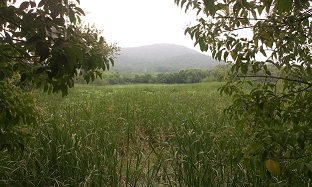
\includegraphics[width=0.7\textwidth]
  {IMAG1097.jpg}

图:雾气朦胧的安徽合肥大蜀山森林公园

拍摄于2014.5.31 - 10:44
\end{figure}
\vspp

\vspp

\fengexian

\begin{center}
在五道口也要红专并进、理实交融呀$\sim$
\end{center}

\tableofcontents


\chapter{Hochschild理论}
\begin{center}
“读论文就是将非人话翻译成人话的过程,
写论文就是将人话写成非人话的过程。”

“我写的公式也不一定对。。。但基本上是对的,up to sign”
\end{center}

\section{结合代数的双模、余中心}

我们需要\textbf{代数拓扑}、\textbf{同调代数}、
\textbf{基础范畴论}的预备知识,
并且采用同调代数的标准术语、记号,
诸如链复形、上同调、导出函子等等。
首先介绍基本的记号与概念。

在本课,我们给定一个特征$0$的含幺交换环$K$(例如一个域),
考虑含幺结合$K$-代数$A$(注意$A$未必是交换代数),
并且$A$作为交换环$K$上的模是投射模(projective module)。
\index{projective module\kong 投射模}
$A$的$K$-代数结构给出如下$K$-模同态:
\begin{eqnarray*}
A\otimes_KA        &\rightarrow& A\\
(a_1,a_2)          &\mapsto    & a_1a_2
\end{eqnarray*}
由$A$的结合性,$(a_1a_2)a_3=a_1(a_2a_3)$
对$A$中任意元素$a_1,a_2,a_3$成立.

对于含幺结合$K$-代数$A$,
回顾$A$的\textbf{反代数}(opposite algebra)
\index{opposite algebra\kong 反代数}
$A\op$.反代数$A\op$作为$K$-模与$A$完全相同,记号如下:
\begin{eqnarray*}
\text{id}:A &\rightarrow & A\op\\
x&\mapsto&x\op
\end{eqnarray*}
但是$A\op$具有与$A$“相反”的乘法,
具体地,对于$A\op$中的元素$x\op,y\op$,
成立
$$x\op y\op:=(yx)\op$$

\begin{definition}(包络代数)

对于含幺结合$K$-代数$A$,我们定义$K$-代数$A^e$为
$$A^e:=A\ten_K A\op$$
即$A$与$A\op$的$K$-代数张量积。
称$A^e$为$A$的\textbf{包络代数}(enveloping algebra)。
\index{enveloping algebra}
\end{definition}

容易验证对于任何两个含幺结合$K$-代数$A,B$,总有
$$(A\ten_K B)\op=A\op\ten_{K}B\op$$
从而容易得到
$$(A\op)^e=(A^e)\op$$

对于$K-$代数$A$,回顾
\textbf{双$A-$模}($A$-bimodule)的概念如下:

\begin{definition}对于$K$-代数$A$,
双$A$-模是指如下资料:

(1)$K$-模$M$;

(2)$A$在$M$上的左、右$K$-线性作用,

并且满足相容性:$(a.m).b=a.(m.b)$对任意$m\in M$以及$a,b\in A$成立。
\end{definition}

例如,$A$本身自然有双$A$-模结构,
$A$在其上的左、右作用即为左乘、右乘。
再比如$K$-模张量积$A\ten_KA$具有如下双$A$-模结构:
$$b.(a_1\ten a_2):=(ba_1)\ten a_2$$
$$(a_1\ten a_2).b:=a_1\ten(a_2b)$$
其中$a_1,a_2,b\in A$.

再比如,对于$K$-代数$A$,考虑其对偶
$$A^*:=\Hom(A,K)$$
则$A^*$具有以下的双$A$-模结构:对任意$a,x\in A$以及$f\in A^*$,
$$
  \left\{
    \begin{array}{l}
      (a.f)(x):=f(xa)\\
      (f.a)(x):=f(ax)
    \end{array}
  \right.
$$
容易验证这的确使得$A^*$为双$A$-模。\vs

我们不再回顾左模、右模的概念了,
也不去回顾右模与左模的平衡张量积。

\begin{prop}设$M$为双$A$-模,

(1)$M$可自然地视为左$A^e$-模:
$$(a_1\ten a_2\op).m=a_1.m.a_2$$

(2)$M$可自然地视为右$A^e$-模:
$$m.(a_1\ten a_2\op)=a_2.m.a_1$$
反之,左(右)$A^e$-模也可视为双$A$-模。
\end{prop}

\begin{proof}
容易验证。
\end{proof}

特别地如果$M,N$都是双$A$-模,那么考虑平衡张量积
$M\ten_{A^e}N$,它的双$A$-模结构具体如下:
$$a.(m\ten n)=(a.m)\ten n=m\ten(n.a)$$
$$(m\ten n).b=m\ten (n.b)=(b.m)\ten n$$
对于任何$m\in M,n\in N,a,b\in A$成立。

\begin{definition}(余中心 cocenter)
\index{cocenter\kong 余中心}
对于双$A$-模$M$,称双$A$-模
$$M\ten_{A^e}A$$
为$M$的\textbf{余中心}(cocenter)。
\end{definition}

容易看出,对任意的$m\in M,a\in A$,
在余中心$M\ten_{A^e}A$当中,成立
$$(m.a)\ten 1=m\ten(a.1)=m\ten a=m\ten(1.a)=(a.m)\ten 1$$
从而$(m.a-a.m)\ten 1=0$.
事实上,$M$的余中心具有如下结构:

\begin{prop}
对于双$A$-模$M$,则有如下双$A$-模同构
$$M\ten_{A^e}A\cong M/\{(m.a-a.m)|a\in A,m\in M\}$$
\label{双模的余中心的结构prop}
\end{prop}

\begin{proof}
考虑如下的双$A$-模链复形
$$\p\downdot:A\ten A\ten A\ra A\ten A\ra A\ra 0$$
其中
\begin{eqnarray*}
\p:a_1\ten a_2\ten a_3 &\mapsto& a_1a_2\ten a_3-a_1\ten a_2a_3\\
a_1\ten a_2&\mapsto&a_1a_2
\end{eqnarray*}
容易验证$\p^2$=0(由$A$的结合性),
从而$\p\downdot$为双$A$-模链复形。
并且显然$\p:A\ten A\ra A$是满同态。

断言链复形$\p\downdot$为正合(exact)的。
\index{exact\kong 正合}
事实上,$\p\downdot$到其自身的恒等链映射与零链映射是链同伦的。
我们构造如下的链同伦$h\downdot$:
\begin{eqnarray*}
h:a_1&\mapsto&1\ten a_1\\
a_1\ten a_2&\mapsto&1\ten a_1\ten a_2
\end{eqnarray*}
容易验证,对于任意的$\varphi=a_1\ten a_2\in A\ten A$,成立
\begin{eqnarray*}
   (\p h+h\p)\varphi
&=&(\p h+h\p)(a_1\ten a_2)\\
&=&\p(1\ten a_1\ten a_2)+h(a_1a_2)\\
&=&a_1\ten a_2-1\ten a_1a_2+1\ten a_1a_2\\
&=&a_1\ten a_2=\varphi\\
\end{eqnarray*}
从而对于$\varphi\in A\ten A$,
如果$\p\varphi=0$,那么
$$\varphi=(\p h+h\p)\varphi=\p(h\varphi)$$
这说明链复形$\p\downdot$在$A\ten A$处正合,
因此$\p\downdot$是正合的。\vs

接下来,将函子$M\ten_{A^e}-$作用于链复形
$\p\downdot$,得到如下的双$A$-模链复形:
$$M\ten_{A^e}\p\downdot:
M\ten A\ra M\ra M\ten_{A^e}A\ra 0$$
由张量函子的右正合性,上述链复形也是正合的。
其中注意到双$A$-模同构
\begin{eqnarray*}
M\ten_{A^e}(A\ten A\ten A)&\cong& M\ten A\\
m\ten(a_1\ten a_2\ten a_3)&\mapsto&(a_3.m.a_1)\ten a_2
\end{eqnarray*}
以及双$A$-模同构
\begin{eqnarray*}
M\ten_{A^e}(A\ten A)&\cong& M\\
m\ten(a_1\ten a_2)&\mapsto& a_2.m.a_1
\end{eqnarray*}

于是正合列$M\ten_{A^e}\p\downdot$的边界映射有如下具体表达式:

\begin{eqnarray*}
M\ten_{A^e}\p:
M\ten A&\to& M\\
m\ten A&\mapsto&m.a-a.m
\end{eqnarray*}

从而由正合性,易知
$$M\ten_{A^e}A\cong M/\{(m.a-a.m)|a\in A,m\in M\}$$
\end{proof}

可见,$M$的余中心无非是商掉$M$当中“非交换的部分”
所得到的“交换的部分”,如此望文生义。
例如,如果$A$为交换$K$-代数,
那么$A$本身作为双$A$-模,其余中心为$A$本身.

\section{Hochschild同调}

\begin{definition}(Hochschild 同调)
\index{Hochschild 同调}

对于双$A$-模$M$,以及非负整数$n$,记
$$H_n(A,M):=\Tor_n^{A^e}(M,A)$$
称为$M$的第$n$个Hochschild同调。特别地,我们记
$$\HH_n(A):=H_n(A,A)$$
\end{definition}

由定义以及导出函子的基础知识,容易知道
双$A-$模$M$的第$0$个Hochschild同调
$$H_0(A,M)=M\ten_{A^e}A=M/\{(m.a-a.m)|a\in A,m\in M\}$$
正是$M$的余中心。
注意Hochschild同调一般并不是环,
仅仅能保证它是双$A$-模。

%%%%%%%%%%%%%%%%2019.2.26 - 第1周第2次%%%%%%%%%%%%%%%%%%%%%%

具体地,由导出函子的定义,
我们采用投射消解(projective resolution)
\index{projective resolution\kong 投射消解}
来计算Hochschild同调。
若双$A$-模链复形
$$P\downdot\to A:=
...\to P_3\to P_2\to P_1\to P_0\to A\to 0$$
为双$A$-模$A$的投射消解
(正合,并且每个$P_i(i\geq 0)$作为$K$-模是投射的),那么
$$H_n(A,M)\cong H_n(M\ten_{A^e}P\downdot)$$
由同调代数的事实,它与投射消解$P\downdot$的选取无关。\vs

事实上Hochschild同调可以与空间上的微分形式类比。
作为一个具体计算例子,我们考虑$\bbC$上的$n$元多项式代数
$$A:=\bbC[x^1,x^2,...,x^n]$$
注意到$A$作为$\bbC$-代数是交换的,从而$A=A\op$.我们记
$$A\op=\bbC[y^1,y^2,...,y^n]\,\,\,\,\,
A^e=\bbC[x^1,x^2,...,x^n;y^1,y^2,...,y^n]$$

\begin{prop}
\label{C[x^i]的HH同调}
考虑$\bbC$-代数$A:=\bbC[x^1,x^2,...,x^n]$,
则其第$k$个Hochschild同调
$$\HH_k(A)\cong\Omg^k_A:=A\ten\wedgeform k(\bbC^n)$$
是以$A$为系数的$k$-形式。
\end{prop}

\begin{proof}

我们给出$A$的投射消解,比如众所周知
的Koszul消解$$\mcalK_A\to A\to 0$$

具体地,引入$n$个新的独立变元
$\eta^1,\eta^2,...,\eta^n$
(视为复线性空间$\bbC^n$的一组基),考虑环
$$\mcalK:=\frac{A^e[\eta^1,\eta^2,...,\eta^n]}
               {\{(\eta^i\eta^j+\eta^j\eta^i)|i\neq j\}}
         =A^e\ten\wedgeform *(\bbC^n)$$
为以$A^e$为系数的外代数。

注意$\mcalK$有自然的分次:
$$\deg\eta^i=1\,\,\,\,\,\deg x^i=\deg y^i=\deg 1=0$$
记$\mcalK_l$为$\mcalK$的$l$次分量($0\leq l\leq n$),即
$$
\mcalK_l=\bigoplus_{1\leq {i_1}<{i_2}<...<{i_l}\leq n}
          A^e\eta^{i_1}\wedge\eta^{i_2}\wedge...\wedge\eta^{i_l}
        =A^e\ten\wedgeform l(\bbC^n)$$
此时$K=\bbC$是域,因此$\mcalK$
(作为$K$-模,即复线性空间)的投射性显然。
我们定义Koszul复形$(\mcalK_A,\p)$如下:
$$\mcalK_A:...\xra{\p} \mcalK_n\xra{\p}\mcalK_{n-1}
\xra{\p}...\xra{\p}\mcalK_1\xra{\p}\mcalK_0$$
其中边缘算子$\p$(首先是$A^e$-模同态)满足

$$\p\eta^i= x^i-y^i$$
以及与外微分相同的莱布尼茨法则:
对任意$\omega\in\mcalK$,成立

$$\p(\eta^i\wedge\omega)=
\p\eta^i\wedge\omega-\eta^i\wedge\p\omega$$

再考虑连接映射
\begin{eqnarray*}
\veps:\mcalK_0=A^c&\to& A\\
x^i&\mapsto&x^i\\
y^i&\mapsto&x^i\\
\end{eqnarray*}
则众所周知,Koszul复形
$$\mcalK_A\xra{\veps} A\to 0$$
为$A$的投射消解(证明从略)。
我们以此计算$\HH\updot(A)$.
我们注意到以下两个简单事实:

其一:对任何$1\leq l\leq n$,
成立双$A$-模同构
$$A\ten_{A^e}\mcalK_l=
A\ten_{A^e}A^e\ten\wedgeform l(\bbC^n)
\cong A\ten\wedgeform l(\bbC^n)$$

其二:函子$A\ten_{A^e}-$作用于Koszul复形
$\mcalK_A$之后,成立
$$A\ten_{A^e}\p=0$$
这是因为,对于任意$f\in A$,在$A\ten_{A^e}A^e$
当中总成立
$$f\ten x^i=x^if\ten 1
=fx^i\ten 1=f\ten (x^i)\op=f\ten y^i$$
因此
$$f\ten(x^i-y^i)=0\in
A\ten_{A^e}A^e$$
从而由$\p$的定义,容易看出$A\ten_{A^e}\p=0$.\vs

综上两方面,直接计算之,
\begin{eqnarray*}
\HH_k(A)&=&H_k(A\ten_{A^e}^LA)\\
&=&H_k(A\ten_{A^e}\mcalK_A)\\
&=&A\ten_{A^e}\mcalK_k\\
&=&A\ten\wedgeform k(\bbC^n)\\
&=&\Omg^k_A
\end{eqnarray*}
从而得证。
\end{proof}

事实上对于一般的含幺结合$K$-代数$A$,$\HH\downdot(A)$
扮演了“微分形式”的角色。这是Hochschild同调的一种几何解释。\vs

对于一般的$A$,
$A$作为双$A$-模,由一种典范的投射消解,
称之为\textbf{Bar-复形}:

\begin{definition}(Bar-复形)

对于含幺结合$K$-代数$A$,定义以下双$A$-模链复形
$$\cdots\to B_2A\xra{b}B_1A\xra{b}B_0A\xra{b}A\to 0$$
如下:
$$B_nA:=A\ten A^{\ten n}\ten A\,\,\,(n\geq 0)$$
\begin{eqnarray*}
b:\,\,a_0\ten a_1\ten...\ten a_n
&\mapsto&
\sum_{k=0}^{n-1}(-1)^k
      a_0\ten a_1\ten...\ten(a_{k}a_{k+1})\ten...\ten a_n
\end{eqnarray*}
称之为\textbf{Bar-复形}。
\index{Bar-复形}
\end{definition}

首先容易验证$b^2=0$,从而
$B\downdot A\xra{b} A\to 0$确实是链复形。
对于$n\geq 1$,具体验证如下:
\begin{eqnarray*}
    b^2(a_0\ten a_1\ten...\ten a_n)
&=& b\left(
         \sum_{k=0}^{n-1}(-1)^k
             a_0\ten a_1
             \ten...\ten(a_{k}a_{k+1})
             \ten...\ten a_n
     \right)\\
&=&  \sum_{k=0}^{n-1}(-1)^k
             b(a_0\ten a_1
             \ten...\ten(a_{k}a_{k+1})
             \ten...\ten a_n)\\
&=&  \sum_{k=0}^{n-1}(-1)^k
         \left[
             \sum_{l=0}^{k-2}(-1)^l
                  a_0\ten...\ten(a_{l}a_{l+1})
                  \ten...\ten(a_{k}a_{k+1})
                  \ten...\ten a_n
         \right.\\
&&+  (-1)^{k-1}
      a_0\ten...\ten(a_{k-1}a_{k}a_{k+1})
                  \ten...\ten a_n\\
&&+
     (-1)^{k}
      a_0\ten...\ten(a_{k}a_{k+1}a_{k+2})
                  \ten...\ten a_n\\
&&-\left.
             \sum_{l=k+2}^{n-1}(-1)^l
                  a_0\ten...\ten(a_{k}a_{k+1})
                  \ten...\ten(a_{l}a_{l+1})
                  \ten...\ten a_n
    \right]\\
&&\\
&=&  \sum_{\substack{0\leq k<l\leq n-1\\ l-k\geq 2}}
         \left(-(-1)^{k+l}+(-1)^{k+l}\right)
         a_0\ten...\ten(a_{k}a_{k+1})
                  \ten...\ten(a_{l}a_{l+1})
                  \ten...\ten a_n\\
&&+  \sum_{0\leq k\leq n-2}
         \left((-1)^{2k+1}+(-1)^{2k}\right)
             a_0\ten...\ten(a_{k}a_{k+1}a_{k+2})
                  \ten...\ten a_n\\
&=&0
\end{eqnarray*}
从而验证完毕。

我们可以把$a_0\ten...\ten a_n$想象为直线上依次排列的$n+1$
个质点,将算子$b$想象为相邻质点两两“碰撞”。

\begin{prop}记号同之前,则Bar-复形
$$B\downdot A\to A\to 0$$
是$A$的投射消解。
\end{prop}

\begin{proof}
对任意$n\geq0$,$B_nA=A\ten A^{\ten n}\ten A$
是投射$K$-模(这是因为由最初的假定,
$A$是投射$K$-模,从而其张量积也投射)
于是我们只需再验证该链复形是正合的。

为此,我们构造链同伦
\begin{eqnarray*}
h:B_{n-2}A&\to& B_{n-1}A
\,\,\,\,\,\,\,(n\geq1,\,B_{-1}A=A)\\
a_0\ten...\ten a_n
&\mapsto&
1\ten a_0\ten...\ten a_n
\end{eqnarray*}

只需验证$hb+bh$=1,
之后与性质\ref{双模的余中心的结构prop}的证明类似。

注意到对于任意$n\geq 0$,成立
\begin{eqnarray*}
    bh(a_0\ten...\ten a_n)
&=& b(1\ten a_0\ten...\ten a_n)\\
&=& a_0\ten...\ten a_n-
    \sum_{k=0}^{n-1}
        1\ten a_0\ten...\ten(a_ka_{k+1})\ten...\ten a_n\\
&=& a_0\ten...\ten a_n-
    1\ten b(a_0\ten...\ten a_n)\\
&=&(1-hb)a_0\ten...\ten a_n
\end{eqnarray*}
因此$bh+hb=1$,证毕。
\end{proof}

\begin{definition}
设$M$为双$A$-模,定义
\textbf{Hochschild链复形}
\index{Hochschild链复形}
\label{Hochschild链复形-def}
$$C\downdot(A,M):=M\ten_{A^e} B\downdot A$$
$$\cdots M\ten A^{\ten 3}\to M\ten A^{\ten 2}\to M\ten A\to M$$
方便起见,该链复形的边缘算子仍记作$b$.
%%%%%%005%%%%%%%
\end{definition}

则易知$M$的Hochdchild同调无非是Hochschlid链复形的同调:
$$H_n(A,M)=H_n(C\downdot(A,M))$$

注意到有双$A$-模同构
$$C_n(A,M)=M\ten_{A^e}
\left(A\ten A^{\ten n}\ten A\right)
\cong M\ten A^{\ten n}$$
在此同构意义下,容易验证$C\downdot(A,M)$
的边缘算子$b$有如下显示表达:

对任意$m\in M$,以及$a_1,a_2,...,a_n\in A$,成立
\begin{eqnarray*}
    b\left(m\ten (a_1\ten...\ten a_n)\right)
&=& m\ten_{A^e}
      \left(
        b(1\ten a_1\ten...\ten a_n\ten 1)
      \right)\\
&=& m\ten_{A^e}
      \large[
        a_1\ten...\ten a_n\ten 1
      \\
&&+  \sum_{k=1}^{n-1}(-1)^k
           1\ten a_1\ten...\ten(a_ka_{k+1})\ten...\ten a_n\ten 1\\
&&+
        (-1)^n1\ten a_1\ten...\ten a_n
    \large]\\
&=& (m.a_1)\ten a_2\ten...\ten a_n\\
&&+ \sum_{k=1}^{n-1}(-1)^k
      m\ten a_1\ten...\ten(a_ka_{k+1})\ten...\ten a_n\\
&&+ (-1)^n(a_n.m)\ten a_1\ten...\ten a_{n-1}
\end{eqnarray*}
Hochschlid链复形的边缘算子的显式表达
与Bar-复形非常相似,从上式最右边的前两项可以看出;
区别在于上式最右边的第三项。\vs

\begin{rem}(Hoschild同调的函子性)
%Functoriality:
若$\fai:A\to B$为$K$-代数同态,
那么$\phi$自然诱导$K$-模同态
$$\fai:\HH\downdot(A)\to \HH\downdot(B)$$
%is a map of $K$-algebra, then
%$$\fai\downdot:C\downdot(A)\to C\downdot(B)$$
%induces
\end{rem}
自行去定义何为$K$-代数同态。此注记表明,
$\HH\downdot$其实是从$K$-代数范畴到$K$-模范畴的一个函子。

\section{Hochschlid上同调}

对于双$A$-模$M$,既然我们已经考虑
余中心$M\ten_{A^e}A$,那么我们自然也会去考虑
$\Hom_{A^e}(A,M)$.我们称
双$A$-模$\Hom_{A^e}(A,M)$为$M$的\textbf{导出中心}
(derived center)。
\index{derived center\kong 导出中心}

\begin{prop}(导出中心的结构)
\label{双模的导出中心的结构prop}
对于双$A$-模$M$,则有双$A$-模同构
$$\Hom_{A^e}(A,M)
\cong\{m\in M|a.m-m.a=0\,\,\,\forall a\in A\}$$
\end{prop}

容易验证$\{m\in M|a.m-m.a=0\,\,\,\forall a\in A\}$
为$M$的双$A$-子模。粗俗地说,
该子模由“与$A$中所有元素交换”的元素构成,
故谓之“中心”。

\begin{proof}对于任意的$\fai\in\Hom_{A^e}(A,M)$
以及$a\in A$,则$\fai(a)$的取值由$\fai(1)$完全决定:
$$\fai(a)=\fai(a.1)=a.\fai(1)$$
而另一方面,
$$\fai(a)=\fai(1.a)=\fai(1).a$$
从而有$a.\fai(1)=\fai(1).a$.
于是我们可以构造如下双$A-$模同态:
\begin{eqnarray*}
\Hom_{A^e}(A,M)
&\to&\{m\in M|a.m-m.a=0\,\,\,\forall a\in A\}\\
\fai&\mapsto&\fai(1)
\end{eqnarray*}
容易验证该模同态为同构。证毕。
\end{proof}

然后我们考虑$\Hom(-,M)$的导出函子,
自然地去定义如下:

\begin{definition}(Hochschild上同调)
\index{Hochschild上同调}
\label{Hochschild上同调-def}

对于双$A$-模$M$,以及$n\geq 0$,
定义$M$的第$n$个Hochschild上同调
$$H^n(A,M)=\Ext_{A^e}^n(A,M)$$
特别地,我们记
$$H^n(A)=\Ext_{A^e}^n(A,A)$$
\end{definition}

由定义知,$M$的第$0$个Hochschild上同调为
$\Hom_{A^e}(A,M)$,是$M$的导出中心。
回顾Bar-复形,我们考虑如下的
\textbf{Hochschild上链复形}
\index{Hochschild上链复形}
$$C\updot(A,M)=\Hom_{A^e}(B\downdot A,M)$$
该上链复形的微分算子$\p$
由Bar-复形$B\downdot A$的边缘算子$b$所诱导。
则$M$的Hochschild上同调满足
$$H^n(A,M)=H^n(C\updot(A,M),\p)
=H^n(\Hom_{A^e}(B\downdot A,M),\p)$$

注意有自然的双$A$-模同构
$$C^n(A,M)
=\Hom_{A^e}(A\ten A^{\ten n}\ten A,M)
\cong\Hom(A^{\ten n},M)$$
(即取值于$M$的$n$重$K$-线性映射)
于是对于任意的$\fai\in C^n(A,M)=\Hom(A^{\ten n},M)$,
容易知道$\p\fai\in\Hom(A^{\ten n+1},M)$具有如下显式表达:
对任意$a_0,a_1,...,a_m\in A$,
\begin{eqnarray*}
    \p\varphi(a_0,a_1,...,a_n)
&=& a_0.\varphi(a_1,a_2,...,a_n)\\
&&- \sum_{k=0}^{n-1}(-1)^k
       \fai(a_0,...;(a_ka_{k+1});...,a_n)\\
&&-  (-1)^n\fai(a_0,a_1,...,a_{n-1}).a_n
\end{eqnarray*}


接下来讨论Hochschild上同调的几何意义。
我们已经知道第0个Hochschild上同调为$M$的导出中心;
现在我们看$H^1(A,M)$,
我们将发现它是$A$的取值于$M$的外导子。

回顾\textbf{导子}(derivation)的概念如下:

\begin{definition}(导子)
对于双$A$-模$M$,$K$-线性映射
$$D:A\to M$$
称为$A$的取值于$M$的\textbf{导子}(derivation),
\index{derivation\kong 导子}
如果对任意的$a_1,a_2\in A$,成立
$$D(a_1a_2)=D(a_1).a_2+a_1.D(a_2)$$
\end{definition}

对于$m\in M$我们定义
\begin{eqnarray*}
\ad_m:A&\to& M\\
a&\mapsto& [m,a]:=m.a-a.m
\end{eqnarray*}
则容易验证$\ad_m$为$A$的取值于$M$的导子,
称形如这样的导子为\textbf{内导子}(inner derivation)。
\index{inner derivation\kong 内导子}

我们记
$$\Der(A,M):=\{D:A\to M|D\text{为导子}\}$$
$$\Inn(A,M):=\{\ad_m|m\in M\}\subseteq \Der(A,M)$$

注意$\Inn(A,M)$与$\Der(A,M)$都有显然的$K$-模结构,
且前者是后者的$K$-子模。

\begin{prop}($H^1(A,M)$的结构)

对于双$A$-模$M$,成立
$$H^1(A,M)\cong\frac{\Der(A,M)}{\Inn(A,M)}$$
\end{prop}
我们称上式右边的集合当中的元素
为$A$的取值于$M$的\textbf{外导子}(outer derivation)。
\index{outer derivation\kong 外导子}

\begin{proof}
只需考虑Hochschild上链复形
$$C^0(A,M)\xra{\p^0}
C^1(A,M)\xra{\p^1}C^2(A,M)\ra\cdots$$

我们只需具体计算之。对于$\fai\in C^1(A,M)\cong\Hom(A,M)$,
则$\p^1\fai\in C^2(A,M)\cong\Hom(A^{\ten 2},M)$满足:
对任意$a_1,a_2\in A$,成立
$$\p^1\fai(a_1,a_2)=
a_1.\fai(a_2)-\fai(a_1a_2)+\fai(a_1).a_2$$
可见$\fai\in\ker\p^1$当且仅当$\fai\in\Der(A,M)$.
也就是说$\ker\p^1=\Der(A,M)$.

另一方面,对于$m\in C^0(A,M)\cong M$,以及$a\in A$,成立
$$(\p^0m)(a)=a.m-m.a=-\ad_m(a)$$
因此$\ker\p^0\cong\Inn(A,M)$.
从而
$$H^1(A,M)=\frac{\ker\p^1}{\im\p^0}
\cong\frac{\Der(A,M)}{\Inn(A,M)}$$
\end{proof}

特别地,当$M=A$时,
$$\HH^1(A)=\Der(A,A)/\text{Inn}(A,A)$$
注意到$\Der(A,A)$上面还有更多的结构:对于
$\forall D_1,D_2\in\Der(A,A)$,定义
$$[D_1,D_2]:=D_1\circ D_2-D_2\circ D_1:A\to A$$
容易验证$[D_1,D_2]$仍然为$A$的导子,并且
$[-,-]$为$\Der(A,A)$上的李括号(Lie bracket)。
\index{Lie bracket\kong 李括号}

另外容易验证
$$[\Der(A,A),\Inn(A,A)]\subseteq\Inn(A,A)$$
具体地,对于$D\in\Der(A,A)$以及$m\in M$,成立
$$[D,\ad_m]=\ad_{D(m)}$$
也就是说$\Inn(A,A)$是$\Der(A,A)$的理想。
于是$[-,-]$诱导了
$\HH^1(A)=\frac{\Der(A,A)}{\text{Inn}(A,A)}$
上的李括号结构.

如果$A$是交换$K$-代数,则$\Inn(A,A)=0$。于是
$$\HH^1(A)\cong\Der(A,A)$$
可被认为是“切向量场”(此时$A$被认为是“函数环”)。

\vsp

我们再去考虑$H^2(A,M)$.对于任意的
$$\varphi\in C^2(A,M)=\Hom(A^{\ten 2},M)$$
则对$a_0,a_1,a_2\in A$,成立
$$\p\varphi(a_0,a_1,a_2)=
a_0.\varphi(a_1,a_2)-\varphi(a_0a_1,a_2)
+\varphi(a_0,a_1a_2)
-\varphi(a_0,a_1).a_2$$

\begin{lemma}对于双$A$-模$M$,以及
$\varphi\in C^2(A,M)=\Hom(A^{\ten 2},M)$,
我们令
$$\Ahat:=A\oplus M$$
并赋以如下的$K$-代数结构:
对于任意$a_1,a_2\in A$以及$m_1,m_2\in M$,
规定$\Ahat$的乘法$\hat{\bullet}_{\fai}$为
$$(a_1\oplus m_1)\hat{\bullet}_{\fai}(a_2\oplus m_2)
:=a_1a_2\oplus [a_1.m_2+m_1.a_2+\fai(a_1,a_2)]$$
那么$(\Ahat,\hat{\bullet}_{\fai})$为结合代数,
当且仅当$\p\fai=0$.
\end{lemma}

\begin{proof}
这是简单的计算验证。对于任意的$a_0,a_1,a_2\in A$
以及$m_0,m_1,m_2\in M$,直接计算之,
\begin{eqnarray*}
&&  [(a_0\oplus m_0)\hat{\bullet}_{\fai}(a_1\oplus m_1)]
    \hat{\bullet}_{\fai}(a_2\oplus m_2)\\
&=& a_0a_1a_2\oplus
    [a_0a_1.m_2+a_0.m_1.a_2+m_0.a_1a_2+
    \fai(a_0,a_1).a_2+\fai(a_0a_1,a_2)]
\end{eqnarray*}
以及
\begin{eqnarray*}
&&  (a_0\oplus m_0)\hat{\bullet}_{\fai}[(a_1\oplus m_1)
    \hat{\bullet}_{\fai}(a_2\oplus m_2)]\\
&=& a_0a_1a_2\oplus
    [a_0a_1.m_2+a_0.m_1.a_2+m_0.a_1a_2+
    a_0.\fai(a_1,a_2)+\fai(a_0,a_1a_2)]
\end{eqnarray*}
因此$\hat{\bullet}_{\fai}$满足结合性,当且仅当
$$\fai(a_0,a_1).a_2+\fai(a_0a_1,a_2)
=a_0.\fai(a_1,a_2)+\fai(a_0,a_1a_2)$$
而此式等价于$\p\fai=0$.
\end{proof}

注意到在$\Ahat$当中,对任意的$m_1,m_2\in M$,
以及任意$\fai\in C^2(A,M)$,
总有$m_1\hat{\bullet}_{\fai}m_2=0$.于是我们不妨将
“$A\oplus M$”当中的“$M$”理解为“一阶小量”。
我们考虑$\fai=0$时$\Ahat_0:=A\oplus M$的代数结构
$$(a_1\oplus m_1)\bullet(a_2\oplus m_2)
:=a_1a_2\oplus (a_1.m_2+m_1.a_2)$$
显然$(\Ahat_0,\bullet)$为结合代数。
若$\p\fai=0$,则结合代数$(\Ahat,\hat{\bullet}_{\fai})$
为$(\Ahat_0,\bullet)$的\textbf{一阶形变},
而$\fai$为其“形变参数”。

从而$M$的第2个Hochschild上同调

$$
    H^2(A,M)\cong
  \frac{
         \{\fai|(\Ahat,\hat{\bullet}_{\fai})
         \text{是结合代数}\}
       }{
       \im(\p:C^1(A,M)\to C^2(A,M))
       }
$$
商掉的东西($\im\p$)为
形如以下的一类特殊的一阶形变:
\begin{eqnarray*}
\fai_f:A\ten A&\to& M\\
a_1\ten a_2 &\mapsto&
a_1.f(a_2)+f(a_1).a_2-f(a_1a_2)
\end{eqnarray*}
其中$f\in C^1(A,M)=\Hom(A,M)$,$\fai_f=\p f$.\vs

Hochschild上同调与Hochschild同调两者之间有如下自然的配对:

\begin{definition}
设$M,N$为双$A$-模,则自然有如下配对:
$$C^n(A,M)\ten C_n(A,N)\to N\ten_{A^e}M$$
定义为:对任意$f\in C^n(A,M)=\Hom(A^{\ten n},M)$
以及任意$y\ten a_1\ten\cdots\ten a_n\in C_n(A,N)=N\ten A^{\ten n}$,
有
$$(f,y\ten a_1\ten\cdots\ten a_n)\mapsto
y\ten f(a_1,...,a_n)\in N\ten_{A^e}M$$
其中任意$y\in N$,以及$a_1,...,a_n\in A$.
\end{definition}

容易验证,该配对自然诱导了
$$H^n(A,M)\ten H_n(A,N)\to N\ten_{A^e}M$$
这是容易发现的(先限制,再下降,下降的良定性容易说明。)

特别地,当$M=A,N=A^*$(其中$A^*:=\Hom(A,K)$)时,
我们有双线性函数
$$H^n(A,A)\ten H_n(A,A^*)\to A^*\ten_{A^e}A\xra{\ev}K$$

%\textbf{Pairing}
%$M,N$ are bi-module,then there is a pairing
%$$C^n(A,M)\ten C_0(A,N)\to N\ten_{A^e}M$$
%So,
%$$H^n(A,M)\ten H_n(A,N)\to N\ten_{A^e}M$$
%$$H^n(A,A^*)\ten H_n(A,A)\to A^*\ten_{A^e}A\xra{ev}K$$

\vs

我们考察一个Hochschild上同调的具体算例。

\begin{prop}若$A=\bbC[x^1,...,x^n]$为
$\bbC$上的$n$元多项式环,则

$$\HH^k(A)\cong
\Hom\left(\wedgeform{k}(\bbC^n),A\right)$$
\end{prop}

\begin{proof}
对于这个特例,采用Koszul复形计算更佳简便。
有关记号同性质\ref{C[x^i]的HH同调}的证明过程.
考虑Koszul复形
$$
\mcalK_A:\cdots
\xra{\p}A^e\ten\wedgeform{k+1}(\bbC^n)
\xra{\p}A^e\ten\wedgeform{k}(\bbC^n)
\xra{\p}A^e\ten\wedgeform{k-1}(\bbC^n)
\xra{\p}\cdots
$$
然后将函子$\Hom_{A^e}(-,A)$作用于之上。
注意到有$\bbC$-线性同构
\begin{eqnarray*}
&&      \Hom_{A^e}\left(A^e\ten\wedgeform{k}(\bbC^n),A\right)\\
&\cong& \Hom\left(\wedgeform{k}(\bbC^n),\Hom_{A^e}(A^e,A)\right)\\
&\cong& \Hom\left(\wedgeform{k}(\bbC^n),A\right)
\end{eqnarray*}

此外再注意到,上链复形$\Hom_{A^e}(\mcalK_A,A)$的
微分算子$\td:=\Hom_{A^e}(\p,A)=0$.这是因为对于
$\fai\in\Hom_{A^e}\left(A^e\ten\wedgeform{k}(\bbC^n),A\right)$,
$\omega\in\wedgeform{k+1}(\bbC^n)$以及$f\in A^e$,成立
$$\td\fai(f\ten\omega)=\fai(\p(f\ten\omega))$$
回顾Koszul复形边缘算子运算规则
$$\p:\eta^i\mapsto x^i-y^i\in A^e$$
又由于$\fai$为$A^e$-模同态,
从而对于任意$\tilde{\omega}\in\wedgeform{k}(\bbC^n)$,成立
$$
\fai(x^i\ten\tilde{\omega})
=x^i.\fai(1\ten\tilde{\omega})
=\fai(1\ten\tilde{\omega}).x^i
=\fai((x^i)\op\ten\tilde{\omega})
=\fai(y^i\ten\tilde{\omega})$$
也就是说$\fai((x^i-y^i)\ten\tilde{\omega})=0$.
由此可见$\td=0$.综上可知

$$\HH^k(A)\cong
\Hom\left(\wedgeform{k}(\bbC^n),A\right)$$

\end{proof}

注意到$\Hom\left(\wedgeform{k}(\bbC^n),A\right)$
之中的元素形如
$$
\sum_{1\leq i_1<...<i_k\leq n}
f_{i_1...i_k}\p_{i_1}\wedge...\wedge\p_{i_k}
$$
回顾$\HH\downdot(A)$中的元素可被认为是“微分形式”,
可见$\HH\updot(A)$中的元素则是“多重切向量场”。



%%%%%%%%%%%2019.3.4 Mon 第2周%%%%%%%%%%%%

\section{约化Bar复形}

如果$K\inj A$为嵌入,那么我们可以更加方便地计算Hochschild
(上)同调:

\begin{definition}(约化Bar-复形)(reduced Bar-complex)
\index{reduced Bar-complex\kong 约化Bar-复形}
\label{约化Bar复形-def}

对于$K$-代数$A$,如果$K\inj A$,那么考虑$K$-模

$$\overline{A}:=A/K$$
我们定义如下的约化Bar-复形$(\overline{B}\downdot A,b)$:
$$\overline{B}_n A:=A\ten \overline{A}^{\ten n}\ten A
\quad \forall \,i\geq 0$$
边缘算子$b:\overline{B}_n A\to \overline{B}_{n-1} A$如下定义:
\begin{eqnarray*}
b\Big(a_0\ten(\overline{a_1}\ten\cdots\ten \overline{a_n})\ten a_{n+1}\Big)
&:=&
 (a_0a_1)\ten(\overline{a_2}\ten\cdots\ten\overline{a_n})\ten a_{n+1}\\
&+ &
 \sum_{i=1}^{n-1}(-1)^ia_0\ten
    (\overline{a_1}\ten\cdots
    (\overline{a_ia_{i+1}})\ten\cdots\ten \overline{a_n})
    \ten a_{n+1}\\
&+ &(-1)^n
 a_0\ten(\overline{a_1}\ten\cdots\ten \overline{a_{n-1}})
   \ten(a_na_{n+1})
\end{eqnarray*}
\end{definition}

注意到$\overline{B}\downdot A$是$B\downdot A$的商模:
$$\overline{B}_nA=
     \frac{B_n A}
     {\{a_0\ten(a_1\ten\cdots
     \ten a_{i-1}\ten 1\ten a_{i+1}
     \ten\cdots\ten a_n)\ten a_{n+1}\}
     }
$$
%%%%%%%%%崩殂%%%%%%!

容易发现约化Bar-复形的“$b$”正是Bar-复形的$b$.
但是我们要验证$b$的良定性,即与代表元选取无关。
这是容易验证的。于是我们得到以下链复形:

$$\overline{B}\downdot A\to A\to 0$$

与之前$Bar$-复形完全类似,我们容易验证此复形也是正合的。
只需构造同伦算子
\begin{eqnarray*}
h:\overline{B}_{n-1}A&\to&\overline{B}_{n}A\\
a_0\ten(\overline{a_1}\ten\cdots\ten \overline{a_{n-1}})\ten a_{n}
&\mapsto&
1\ten(\overline{a_0}\ten\overline{a_1}\ten\cdots\ten \overline{a_n})\ten a_{n+1}
\end{eqnarray*}
验证$bh+hb=1$即可。
%%%%%%天下三分%%%%%%%!

\begin{definition}(约化Hochschild(上)链复形)

对于双$A$-模$M$,我们令
\begin{eqnarray*}
\overline{C}\downdot(A,M)&:=&
M\ten_{A^e}\overline{B}\downdot A\cong M\ten\overline{A}^{\ten\bullet}\\
\overline{C}\updot(A,M)&:=&
\Hom_{A^e}(\overline{B}\downdot A,M)
\cong\Hom(\overline{A}^{\ten\bullet},M)
\end{eqnarray*}
称之为关于$M$的约化Hochschild(上)链复形。
\end{definition}

事实上,约化Hochschild(上)
链复形的(上)同调自然同构于Hochschild(上)同调——
这是由以下代数引理保证的:

\begin{lemma}条件同上,则商映射
$$\pi\downdot:C\downdot(A,M)
\surj\overline{C}\downdot(A,M)$$
所诱导的链映射
$$\pi\downdot:(C\downdot(A,M),d)
\surj(\overline{C}\downdot(A,M),d)$$
为拟同构。
\label{约化Hoschild复形与拟同构-lemma}
\end{lemma}

\begin{proof}
注意链映射$\pi\downdot$为满态射,
只需再证明其核复形
$$\ker\pi\downdot$$
是正合的即可。我们承认之(似乎不太好证)。
\end{proof}

注意上述引理也适用于Hochschild上链复形的情形,
完全类似,不再赘述。
从而我们立刻有如下推论:

\begin{cor}
对于$K$-代数$A$,如果$K\inj A$为嵌入,则有自然同构:
\begin{eqnarray*}
H\downdot(A,M)&\cong&H\downdot(\overline{C}\downdot(A,M))\\
H\updot  (A,M)&\cong&H\updot  (\overline{C}\updot  (A,M))
\end{eqnarray*}
\end{cor}

关于(约化)Bar-复形,我们还有另一种理解方式:
关于$A$的(约化)Bar-复形是$A$与某个微分分次代数的自由乘积。
%Another way to understand $B\downdot A,\bar{B}\downdot A$

\begin{definition}(微分分次代数)

%A differential graded algebra
\index{differential graded algebra\kong 微分分次代数}
$\bbZ$-分次$K$-代数
$$A:=\bigoplus_{n\in\mathbb{Z}}A_n$$
称为\textbf{微分分次代数}(differential graded algebra),
若它配以$K$-线性算子$\td:A\to A$,并且满足:
$$\left\{\begin{array}{l}
\td(A_n)\subseteq A_{n+1}\quad\forall n\in\bbZ\\
\td^2=0\\
\td(\alpha\beta)
=(\td\alpha)\beta+(-1)^{\deg\alpha}\alpha(\td\beta)
\quad\forall\alpha,\beta\in A\text{,并且$\alpha$是齐次元}
\end{array}\right.$$
\label{微分分次代数-def}
\end{definition}

“$\bbZ$-分次$K$-代数”的定义
将在后文(定义\ref{分次结合代数-def})介绍。
(其实大家都明白)

对于微分分次代数$(A,\td)$,由于$A$的分次以及$\td^2=0$,
从而自然有上链复形
$$\cdots\to A_{-1}\xra{\td}A_0\xra{\td}A_1\to\cdots$$
我们将此上链复形也记为$(A,\td)$.

微分分次代数最直接的例子是,对于光滑流形$X$,
考虑$A:=\Omg\updot(X)$为$X$上的微分形式。
$A$上的乘法即为微分形式的外积$\wedge$,
微分结构即为外微分$\td$.

我们可以适当修改微分分次代数的定义,
将条件“$\td(A_n)\subseteq A_{n+1}$”改为
“$\td(A_n)\subseteq A_{n-1}$”,
此时的微分算子我们习惯记为“$\p$”.
对于这样的微分分次代数$(A,\p)$,它可以被视为链复形。

\begin{example}我们考虑如下$K$-代数:
$$A:=K[\veps]:=K\oplus K\veps\oplus K\veps^2\oplus\cdots$$
其中$\veps$为形式变量,并且规定$\deg\veps=1$,
由此诱导出$K[\veps]$的分次结构。其微分算子$\p_{\veps}$由以下诱导:
$$\p_{\veps}(1)=0\quad\p_{\veps}(\veps)=1$$
\label{典型微分分次代数-example}
\end{example}

注意$\deg\veps=1$,按照微分代数的定义可计算出
$$\p_{\veps}(\veps^2)=
  \p_{\veps}(\veps)\veps
  +(-1)^{\deg\veps}\veps\p_{\veps}(\veps)
=\veps-\veps=0$$
一般地,对于非负整数$n$我们有
$$
  \p_{\veps}(\veps^n)
= \left\{
    \begin{array}{ll}
      0           &\text{$n$为偶数}\\
      \veps^{n-1} &\text{$n$为奇数}
    \end{array}
  \right.
$$
从而链复形$(K[\veps],\p_{\veps})$:
$$\cdots\to K\veps^4\xra{0}K\veps^3\xra{1}
K\veps^2\xra{0}K\veps\xra{1}K\to 0$$
是正合的。其中$1:K\veps^{2n+1}\to K\veps^{2n}$
将$\veps^{2n+1}$映为$\veps^{2n}$.

%%%%微分分次代数的例子%%%%%%%!

众所周知,对于两个$K$-代数$A,B$,
我们可以谈论它们的\textbf{自由乘积}(free product)
$A*B$.若$A=\bigoplus\limits_{i\in\bbZ}A_n$是微分分次代数,
其微分算子为$\td$,则容易知道$A*B$自然也有微分分次代数结构:
$$
\left\{
    \begin{array}{rcll}
       \deg b&=&0&\forall{b\in B}\\
       \deg a&=&n&\forall{a\in A_n\subseteq A}\\
       \td b&=&0 &\forall{b\in B}
    \end{array}
\right.
$$
容易知道$A*B$中的$N$次齐次元必形如以下元素的有限和:
$$b_1a_1b_2a_2\cdots b_ma_mb_{m+1}\quad
(b_i\in B\,,\,a_i\in A_{n_i}\,,\,\sum_{i=1}^mn_i=N)$$

\begin{prop}
对于$K$-代数$A$,则有链复形的同构
$$(B\downdot A\to A,b)\cong (A*K[\veps],\p_{\veps})$$
其中$(K[\veps],\p_{\veps})$为例子
\ref{典型微分分次代数-example}
当中的微分分次代数,视为链复形;
同构映射为
\begin{eqnarray*}
\fai_n:B_nA&\to&(A*K[\veps])_n\\
a_0\ten(a_1\ten\cdots\ten a_n)\ten a_{n+1}&\mapsto&
a_0\veps a_1\veps a_2\cdots a_n\veps a_{n+1}
\end{eqnarray*}
%the bar resolution $[B\downdot\to A]\cong A*K[\veps]$
%(free product),and $b=\p_{\veps}$
\end{prop}

这给出了Bar-复形的又一种理解方式。

\begin{proof}
容易验证$\fai_n$为$K$-模同构,且逆映射$\fai_n^{-1}$由以下诱导:
$$\veps^n\mapsto\underbrace
{1\veps 1\veps 1\cdots 1\veps 1}_{n\text{个}\veps}$$
然后只需验证$\fai\downdot:(B\downdot\to A,b)\to(A*K[\veps],\p_{\veps})$:
是链映射,也就是要验证交换关系$\fai\circ b=\p_{\veps}\circ\fai$
$$
\xymatrix{
B_nA \ar[d]^{\fai} \ar[r]^b         &B_{n-1}A\ar[d]^{\fai}\\
(K[\veps]*A)_n \ar[r]^{\p_{\veps}}  &(K[\veps]*A)_{n-1}
}$$
而这容易验证,验证如下:
\begin{eqnarray*}
&&   \fai\circ b(a_0\ten a_1\ten\cdots\ten a_n\ten a_{n+1})\\
&= &\fai\left(
          \sum_{k=0}^n(-1)^k
            a_0\ten\cdots\ten(a_k a_{k+1})\ten\cdots\ten a_{n+1}
       \right)\\
&= &\sum_{k=0}^n(-1)^k
      a_0\veps a_1\veps\cdots\veps a_{n+1}\\
&= &\p_{\veps}(a_0\veps a_1\veps\cdots a_n\veps a_{n+1})\\
&= &\p_{\veps}\circ\fai(a_0\ten a_1\ten\cdots\ten a_n\ten a_{n+1})
\end{eqnarray*}

%$$[B\downdot A\to A]\mapsto A*K[\veps]$$
%$$a_0\ten...\ten a_n\mapsto
%a_0\veps a_1\veps...a_{n-1}\veps a_n$$
%this is bijective.

%$$\p_{\veps}:a_0\veps a_1\veps...a_{n-1}\veps a_n\mapsto
%a_0a_1\veps.....-a_0\veps a_1a_2...$$
%...

%check

\end{proof}

我们还可以考虑$(K[\veps],\p_{\veps})$的商代数
$K[\veps]/\veps^2$,易知
$(K[\veps]/\veps^2,\p_{\veps})$也构成微分分次代数,
从而也通过微分算子$\p_{\veps}$视为链复形。
在此代数中,$\veps^2=0$.\vs

类似地,我们可以给出约化Bar-复形的另一种理解方式:

\begin{prop}
对于$K$-代数$A$,则有链复形同构
$$(\overline{B}\downdot A\to A,b)\cong (A*K[\veps]/\veps^2,\p_{\veps})$$
\end{prop}

只需注意到$A*K[\veps]/\veps^2$
当中的$n$次齐次元必形如以下元素的有限和:
$$a_0\veps a_1\veps\cdots a_n\veps a_{n+1}\quad (a_i\in A)$$

\begin{proof}
完全类似。事实上此链复形同构映射由
$\fai_n:B_nA \to (A*K[\veps])_n$诱导,
其良定性由下式保证:对任意$1\leq i\leq n$,
\begin{eqnarray*}
&&  \fai_n(a_0\ten \cdots\ten a_{i-1}
    \ten 1\ten a_{i+1}\ten\cdots\ten a_{n+1})\\
&=& a_0\veps a_1\cdots a_{i-1}\veps1\veps a_{i+1}\cdots\veps a_{n+1}\\
&=& a_0\veps a_1\cdots a_{i-1}1\veps^2a_{i+1}\cdots\veps a_{n+1}\\
&=& 0\mod\veps^2
\end{eqnarray*}
\end{proof}
%Similarly, reduced Bar-complex
%$$[\bar{B}\downdot A\to A]\cong A*K[\veps]/\veps^2$$

本节最后简单介绍以下Hochschild(上)
同调与其它常见的(上)同调理论的关系。

\begin{example}(群的上同调)%(Group (co)homology)

设$G$是一个群,$M\in\Rep(G)$为群$G$的一个左$K$-表示,
则有$G$-模链复形
%Let $G$ be a group, $M\in\text{Rep}(G)$ is a left module,
%then we obtain a complex
$$0\to M\xra{\delta}C^1(G,M)\xra{\delta}C^2(G,M)\xra{\delta}...$$
其中%where
$$C^n(G,M):=\Hom(G^n,M)=\{f:G^n\to M\}$$
并且微分算子$\delta$满足%the differential $\delta$ s.t.
$$\left\{\begin{array}{rcl}
\delta(m)(g)&=&g.m-m\\
(\delta f)(g_0,g_1,...,g_n)&=&
g_0.f(g_1,g_2,...,g_n)\\
&&-\sum\limits_{k=1}^{n-1}(-1)^kf(g_1,...,g_kg_{k+1},...,g_n)\\
&&-(-1)^nf(g_0,g_1,...,g_{n-1})
\end{array}\right.
$$
%check $\delta^2=0$,this cohomology
容易验证$\delta^2$=0.此链复形的上同调
$$H\updot(G,M):=H\updot(C\updot(G,M),\delta)$$
称之为\textbf{群的上同调}(group cohomology)
\index{group cohomology\kong 群的上同调}
\end{example}

由$\delta$的表达式容易看出,
群的上同调与Hochschild上同调有以下关系:

\begin{prop}设$G$是一个群,$M$为群$G$的一个左$K$-模,
考虑群代数$A:=K[G]$,于是$M$自然有左$A$-模结构。那么有同构:
%Let $A=K[G]$ group algebra with right $A$-action.then
$$H\updot(G,M)\cong H\updot(K[G],M)$$
%hochschild cohomology.
其中左边为群$G$关于$M$的上同调,
右边为群代数$K[G]$关于$M$的Hichschild上同调。
\end{prop}

{\color{red}
注意$M$仅仅是左$K[G]$-模,并没有双$K[G]$-模结构呀,
怎么谈论Hochschild上同调?

\color{purple}
(强行规定$G$在$M$上的右作用恒为1,
通过$K$-线性扩张得到$K[G]$在$M$的右作用,
这样就得到$M$的双$K[G]$-模结构了。)}

\begin{proof}
注意到$\Hom(G^n,M)$中的元素可以自然地$K$-线性延拓为
$\Hom(K[G]^n,M)$中的元素,这给出它们之间的同构。
然后注意到$A=K[G]$的Hochschild上链复形的微分算子的显式表达式,
(见定义\ref{Hochschild上同调-def}的下方)
它与群上同调相应的上链复形的微分算子显式表达式
“相同”。细节从略。
\end{proof}

若熟悉李代数同调,我们可以将李代数同调与
其泛包络代数的Hochschild同调联系起来:

\begin{example}(李代数同调)%(Lie algebra (co)homology)
对于李代数$\mfkg$,$M$为李代数$\mfkg$的一个左$K$-模。
令$A:=\mcalU(\mfkg)$为$\mfkg$的泛包络代数,
则$A$自然有左$A$-模结构。
(再通过某种“比较平凡”的方式给出右作用?与上例类似?)
则有同构
%$\mathfrak{g}$:Lie algebra, $M$ is a $\mathfrak{g}$-module.
%consider $A:=\mathcal{U}(\mathfrak{g})$ universal enveloping algebra,
%$M$ is a left $A$-module, with
$$H\downdot(\mathcal{U}(\mathfrak{g}),M)
\cong H^{\Lie}\downdot(\mathfrak{g},M)$$
其中左边是$A$关于$M$的Hochschild同调,右边是李代数同调。
\end{example}

并没有在此叙述\textbf{李代数同调}的定义。
留给感兴趣者。此处从略。

事实上,也可以考虑\textbf{群的同调}、\textbf{李代数上同调},
它们也有对应的Hochschild同调、上同调。



\section{Connes复形$C^{\lmd}\downdot(A)$}
%Cyclic homology%
%$\HH\downdot(A)\rightsquigarrow$noncommutative differential forms.
%$$B\dashleftarrow\text{de rham}$$

与之前一样,我们仍假设$K$为特征零的含幺交换环,
$A$为$K$-代数,且作为$K$-模是投射的。
不过,在从本节开始我们再新增一条假定:
$$\bbQ\inj K$$
也就是说,有理数域能够嵌入到$K$中。
(事实上,任何特征零的域都满足此假定。)

回顾对于$K$-代数$A$,若$A$交换,
则其Hochschild同调$\HH\downdot(A)$
可以被理解为“空间”$A$上的“微分形式”。
本节我们进一步研究$\HH\downdot(A)$.

\begin{notation}
对于$K$-代数$A$,双$A$-模$M=A$.
考虑其Hochschild链复形$C\downdot(A):=C\downdot(A,A)$:
$$C_n(A):=C_n(A,A)\cong A^{\ten n+1}$$
(回顾定义\ref{Hochschild链复形-def}).我们考虑群
$\bbZ/(n+1)\bbZ$在$C_n(A)$上的如下左$K$-作用:
记$\bbZ/(n+1)\bbZ$的生成元为$\lmd$,则
\begin{eqnarray*}
\lmd:C_n(A)&\to&C_n(A)\\
a_0\ten a_1\ten\cdots\ten a_n
&\mapsto&
(-1)^na_n\ten a_0\ten\cdots\ten a_{n-1}
\end{eqnarray*}
考虑$C_n(A)$模掉此群作用,所得的商$K$-模记为
$$C^{\lmd}_n(A):=C_n(A)/(1-\lmd)$$
其中的元素称之为\textbf{循环余不变量}
(cyclic co-invariant)。
\index{cyclic co-invariant\kong 循环余不变量}
\end{notation}

%cyclic group action
%$$C\downdot(A,A)=C\downdot(A)=A\ten A$$
%$$C_n(A)=A^{\ten n+1}$$
%we consider the $\bbZ/(n+1)\bbZ$ acting on $C_n A$,
%$$\lmd: C_n(A)\to C_n(A)$$
%$$a_0\ten a_1\ten...\ten a_n\mapsto
%(-1)^na_n
%\ten a_0\ten...\ten a_{n-1}$$
%then $\lmd$ is generator,
%$$\lmd^{n+1}=(-1)^{n(n+1)}=1$$
%Let
%$$C^{\lmd}\downdot(A):=C\downdot(A)/(1-\lmd)$$
%cyclic co-invariant.

容易验证,
$$\lmd^{n+1}a_0\ten a_1\ten\cdots\ten a_n=
(-1)^{n(n+1)}a_0\ten a_1\ten\cdots\ten a_n
=a_0\ten a_1\ten\cdots\ten a_n$$
即$\lmd^{n+1}=\id$.可见这的确是$\bbZ/(n+1)\bbZ$的作用。

回顾Bar-复形,我们可以直观地视为“直线上依次排列质点,相邻两两碰撞”;
而在这里,商掉$\lmd$循环作用后,直观地更像是“圆周上排列质点”。

我们将说明,Hochschild链复形$C\downdot(A)$的边缘算子$b$,
沿商映射$C\downdot(A)\surj C^{\lmd}\downdot(A)$下降,诱导了
$C\downdot^{\lmd}(A)$的链复形结构(称之为Connes复形)。

%\begin{prop}
%对于$K$代数$A$,定义$b‘:C_{n}(A)\to C_{n-1}(A)$诱导了
%$C^{\lmd}\downdot$的链复形结构。
%Hochschild differential $b$(on $C\downdot(A)$) induces a
%differential on $C\downdot(A)/(1-\lmd)$
%\end{prop}

%\begin{proof}

%事实上,我们定义$b‘:C^{\lmd}_n(A)\to C_n^{\lmd}(A)$如下:
%\begin{eqnarray*}
%b’:C^{\lmd}_n(A)&\to& C_n^{\lmd}(A)\\
%\overline{
%   a_0\ten a_1\ten\cdots\ten a_n
%         }
%&\mapsto&
%   \sum_{k=0}^{n-1}(-1)^k
%       \overline{
%         a_0\ten\cdots\ten(a_ka_{k+1})\ten\cdots a_n
%       }\\
%&&
%   +(-1)^n\overline{
%     (a_{n+1}a_0)\ten a_1\ten\cdots\ten a_n
%         }
%\end{eqnarray*}
%即$b:C_n(A)\to C_{n-1}(A)$沿商映射的下降。
%(回顾Hochschild链复形的边缘算子$b$的显式表达,见
%定义\ref{Hochschild链复形-def}的下方,令$M=A$以及$m=a_0$.)

%我们需要验证如此$b'$是良定的,
%即与$\lmd$作用等价类代表元选取无关。
%{\color{purple}(直观感觉比较显然,但还是暴力验证一下吧)}

%Let us define
%$$b':C\downdot(A)\to C_{\bullet-1}(A)$$
%$$b'(a_0\ten...\ten a_n)
%=a_0a_1\ten a_2\ten...\pm...\pm a_0\ten a_1\ten...\ten a_{n-1}a_n$$

%(($C\downdot(A),b')=(B\downdot A\to A)$)

%claim that
%$$(1-\lmd)b'=b(1-\lmd)$$

%$$[b,\lmd]=(1-\lmd)(b-b')$$

%In particular, $b:\im(1-\lmd)\mapsto\im(1-\lmd)$

%"proof":
%%%%%%%%%%画圈圈%%%%%%%%%%%555

%为此只需验证对于任意$n\geq 1$,以及任意$\omg\in C_n(A)$,
%$$(1-\lmd)(\omg)=0\Rightarrow(1-\lmd)\circ b(\omg)=0$$

%\end{proof}

\begin{lemma}
对于$K$-代数$A$,我们定义算子
$b':C\downdot(A)\to C_{\bullet-1}(A)$如下:
\begin{eqnarray*}
b':C_{n}(A)&\to&C_{n-1}(A)\\
a_0\ten a_1\ten\cdots\ten a_n&\mapsto&
\sum_{k=0}^{n-1}(-1)^{k}
a_0\ten\cdots\ten(a_ka_{k+1})\ten\cdots\ten a_n
\end{eqnarray*}
则成立:

(1)$b'\circ b'=0$,

(2)对任意$n\geq 1$,则以下图表交换:
$$\xymatrix{
     C_n(A) \ar[d]^{1-\lmd} \ar[r]^{b'}
   & C_{n-1}(A)\ar[d]^{1-\lmd}
\\
     C_n(A) \ar[r]^b
   & C_{n-1}(A)
}$$
\end{lemma}

\begin{proof}
注意到有同构$C_n(A)\cong B_nA(\cong A^{\ten n+1})$,
其中$B\downdot A$为Bar-复形;容易看出这里定义的$b'$在此同构下,正是
Bar复形当中的边缘算子,从而$b'\circ b'=0$,
也就是说$(C\downdot(A),b')$是一个链复形,
并且同构于Bar-复形$(B\downdot A, b)$.
(这里有轻微的记号混用:Bar-复形$(B\downdot A, b)$当中的“$b$”
并不是本引理当中Hochschild链复形$(C\downdot(A),b)$当中的“$b$”,
前者在此是临时记号。)\vs

我们再来看(2).回顾$b:C_n(A)\to C_{n-1}(A)$的显式表达式
(见定义\ref{Hochschild链复形-def}的下方,并且令其中$M=a$以及$m=a_0$)
(注意此图中的$b$与$b'$并不是同一个映射,它们的具体表达式相差一项),
直接验算之:
\begin{eqnarray*}
& & (1-\lmd)\circ b'
        \big(
             a_0\ten a_1\ten\cdots\ten a_n
        \big)\\
&=&
    (1-\lmd)\left(
               \sum_{k=0}^{n-1}(-1)^k
                   a_0\ten\cdots\ten(a_ka_{k+1})\ten\cdots\ten a_n
            \right)\\
&=&
    \sum_{k=0}^{n-1}(-1)^k
         a_0\ten\cdots\ten(a_ka_{k+1})\ten\cdots\ten a_n\\
& &
    +\sum_{k=0}^{n-2}(-1)^{k+n}
         a_n\ten a_0\ten\cdots\ten(a_ka_{k+1})\ten\cdots\ten a_{n-1}\\
& &
    -(a_{n-1}a_n)\ten a_0\ten\cdots\ten a_{n-2}\\
&=&
    b(a_0\ten a_1\ten\cdots\ten a_n)
    -(-1)^n(a_na_0)\ten a_1\ten\cdots\ten a_{n-1}\\
& &
    +(-1)^n
    \sum_{k=0}^{n-1}(-1)^k
        a_n\ten a_0\ten\cdots\ten(a_ka_{k+1})\ten\cdots\ten a_{n-1}\\
& &
    -(a_{n-1}a_n)\ten a_0\ten\cdots\ten a_{n-2}\\
&=&
    b\big(
       a_0\ten a_1\ten\cdots\ten a_n
       -(-1)^na_n\ten a_0\ten\cdots\ten a_{n-1}
     \big)\\
&=&
    b\circ(1-\lmd)(a_0\ten a_1\ten\cdots\ten a_n)
\end{eqnarray*}

也就是说,
$$(1-\lmd)\circ b'=b\circ(1-\lmd)$$
从而此图表交换,证毕。
\end{proof}

此图表的交换关系也可改写为
$$[b,\lmd]=(1-\lmd)\circ(b-b')$$
其中$[b,\lmd]:=b\circ\lmd-\lmd\circ b$.\vs

此引理给出了链复形$(C\downdot(A),b')$与
$(C\downdot(A),b)$之间的链映射:
$$(1-\lmd)\downdot:(C\downdot(A),b')\to(C\downdot(A),b)$$
然而注意到
$$C_n^{\lmd}(A):=C_n(A)/(1-\lmd)=\coker (1-\lmd)_n$$
于是我们(在由$K$-模链复形构成范畴当中)
考虑链映射$(1-\lmd)\downdot$的余核,
这给出了$C\downdot^{\lmd}(A)$的链复形结构:

\begin{definition}(Connes复形)
\index{Connes' complex\kong Connes复形}
对于$K$-代数$A$,考虑链映射
$$(1-\lmd)\downdot:(C\downdot(A),b')\to(C\downdot(A),b)$$
的余核链复形
$$(C\downdot^{\lmd}(A),b^{\lmd}):=\coker[(1-\lmd)\downdot]$$
称其为\textbf{Connes复形}。并且记
$$H^{\lmd}\downdot(A):=H\downdot(C\downdot^{\lmd}(A))$$
称之为$A$的\textbf{循环同调}(cyclic homology).
\index{cyclic homology\kong 循环同调}
\end{definition}

也就是说,有如下的交换图表:

$$\xymatrix{
     \cdots \ar[r]
   & C_{n+1}\ar[r]^{b'}  \ar[d]^{1-\lmd}
   & C_{n  }\ar[r]^{b'}  \ar[d]^{1-\lmd}
   & C_{n-1}\ar[r]       \ar[d]^{1-\lmd}
   & \cdots
\\
     \cdots \ar[r]
   & C_{n+1}\ar[r]^{b }  \ar@{->>}[d]
   & C_{n  }\ar[r]^{b }  \ar@{->>}[d]
   & C_{n-1}\ar[r]       \ar@{->>}[d]
   & \cdots
\\
     \cdots \ar[r]
   & C_{n+1}^{\lmd}\ar[r]^{b^{\lmd}} \ar[d]
   & C_{n  }^{\lmd}\ar[r]^{b^{\lmd}} \ar[d]
   & C_{n-1}^{\lmd}\ar[r]            \ar[d]
   & \cdots
\\
   &0
   &0
   &0
   &
}$$
此交换图表每一横行都为链复形,其中第三横行为Connes复形;
每一列都是右短正合的。
并且容易知道:Connes复形的边缘算子$b^{\lmd}$
正是Hochschild链复形的边缘算子$b$沿商映射
$C\downdot(A)\surj C^{\lmd}\downdot(A)$的下降。

%so, $b$ acts on $C^{\lmd}\downdot(A)=C\downdot(A)/(1-\lmd)$
%,called \textbf{Connes' complex}
%$$H^{\lmd}\downdot(A)=H\downdot(C^{\lmd}\downdot(A),b)$$

\section{循环双复形$CC\ddowndot(A)$}

\begin{lemma}(平均算子)对于任意$K$-代数$A$,以及$n\geq 0$,
引入平均算子$\mathcal{N}:C_n(A)\to C_n(A)$:
$$\mcalN:=1+\lmd+\lmd^2+\cdots+\lmd^n$$
则此算子满足以下性质:

(1)$b'\mcalN=\mcalN b$

(2)$(1-\lmd)\mcalN=\mcalN(1-\lmd)=0$.
此外,如果有理数域$\bbQ\hookrightarrow K$,
那么对于任意$n\geq 0$,以下链复形是正合的:
$$\cdots\to
C_n(A)\xra{\mcalN}C_n(A)\xra{1-\lmd}
C_n(A)\xra{\mcalN}C_n(A)\xra{1-\lmd}
C_n(A)\surj C_n^{\lmd}(A)\to 0
$$
%Introduce
%$$\mathcal{N}:C_n(A)\to C_n(A)$$
\label{循环双复形的行正合性-lemma}
\end{lemma}
%%%%%%%%%%%平均算子%%%%%%%%%'

%\begin{prop}
%$$b'\mathcal{N}=Nb$$
%\end{prop}

%we have an exact sequence
%%%%%%%平均算子‘%%%%%%'
\begin{proof}(1)任意固定$n\geq 1$,
为了区分算子在不同空间的作用,
我们采用临时记号
$$\left\{\begin{array}{l}
\lmd:C_n(A)\to C_n(A)\\
\overline{\lmd}:C_{n-1}(A)\to C_{n-1}(A)
\end{array}\right.\quad
\left\{\begin{array}{l}
\mcalN:=1+\lmd+\cdots+\lmd^n\\
\overline{\mcalN}:=1+\overline{\lmd}+\cdots+\overline{\lmd}^{n-1}
\end{array}\right.$$
则在此记号下我们需要证$b'\mcalN=\overline{\mcalN}b$.

定义缩并算子
\begin{eqnarray*}
s:C_n(A)&\to& C_{n-1}(A)\\
a_0\ten a_1\ten\cdots\ten a_n
&\mapsto&
(a_0a_1)\ten\cdots\ten a_n
\end{eqnarray*}
则容易验证(稍微注意一下正负号,确实都是正号)
$$
b =\sum\limits_{k=0}^n    \overline{\lmd}^ks\lmd^{-k}\quad\quad
b'=\sum\limits_{k=0}^{n-1}\overline{\lmd}^ks\lmd^{-k}
$$
于是有
$$
b'\mcalN=
  \left(
    \sum_{k=0}^{n-1}
      \overline{\lmd}^ks\lmd^{-k}
  \right)
  \left(
    \sum_{l=0}^{n  }
      \lmd^l
  \right)
=
 \sum_{0\leq k\leq n-1
       \atop
       0\leq l\leq n}
     \overline{\lmd}^ks\lmd^l
$$
同理也有
$$\overline{\mcalN}b
=\sum_{0\leq k\leq n-1
       \atop
       0\leq l\leq n}
     \overline{\lmd}^ks\lmd^l$$
从而$b'\mcalN=\overline{\mcalN}b$.

(2)给定$n\geq 0$,注意到$\lmd^{n+1}=1$,从而
$$(1-\lmd)\mcalN=(1-\lmd)(1+\lmd+\cdots+\lmd^n)=1-\lmd^{n+1}=0$$
同理$\mcalN(1-\lmd)=0$.因此该图表是链复形,只需再验证正合性。

现在假设$\bbQ$是$K$的子环。我们构造如下链同伦:

$$\xymatrix{
   \cdots \ar[r]
  &C_n(A) \ar[r]^{\mcalN} \ar[d]^{\id}
  &C_n(A) \ar[r]^{1-\lmd} \ar[d]^{\id} \ar[ld]_g
  &C_n(A) \ar[r]^{\mcalN} \ar[d]^{\id} \ar[ld]_f
  &C_n(A) \ar[r]^{      } \ar[d]^{\id} \ar[ld]_g
  &\cdots
\\
   \cdots \ar[r]
  &C_n(A) \ar[r]^{\mcalN}
  &C_n(A) \ar[r]^{1-\lmd}
  &C_n(A) \ar[r]^{\mcalN}
  &C_n(A) \ar[r]^{      }
  &\cdots
}$$
其中$f,g:C_n(A)\to C_n(A)$定义为
$$\left\{\begin{array}{l}
f:=\frac{1}{n+1}(\lmd^{n-1}+2\lmd^{n-2}+3\lmd^{n-3}+\cdots+n)\\
g:=\frac{1}{n+1}
\end{array}\right.$$
(利用了$\bbQ\inj K$)则容易验证
$$f(1-\lmd)+\mcalN g=g\mcalN+(1-\lmd)f=1$$
从而证毕。
\end{proof}

特别地,当$K$为域时(注意我们总假定$\ch K=0$)成立正合性。
链同伦$f,g$的构造来自于(关于变元$\lmd$的多项式的)
欧几里得辗转相除法。

%\begin{definition}
%the cyclic bi-complex $CC\downdot(A)$
%%%%%%%双复形%%%%%%
%\end{definition}

由此引理,我们可构造出如下的\textbf{循环双复形}
(cyclic bicomplex),记为$CC\ddowndot(A)$:
\index{cyclic bicomplex\kong 循环双复形}

$$\xymatrix{
   \vdots \ar[d]^b
  &\vdots \ar[d]^{-b'}
  &\vdots \ar[d]^b
  &\vdots \ar[d]^{-b'}
  &
\\
   C_2(A) \ar[d]^b
  &C_2(A) \ar[d]^{-b'} \ar[l]_{1-\lmd}
  &C_2(A) \ar[d]^b     \ar[l]_{\mcalN}
  &C_2(A) \ar[d]^{-b'} \ar[l]_{1-\lmd}
  &\cdots              \ar[l]
\\
   C_1(A) \ar[d]^b
  &C_1(A) \ar[d]^{-b'} \ar[l]_{1-\lmd}
  &C_1(A) \ar[d]^b     \ar[l]_{\mcalN}
  &C_1(A) \ar[d]^{-b'} \ar[l]_{1-\lmd}
  &\cdots              \ar[l]
\\
   C_0(A)
  &C_0(A)   \ar[l]_{1-\lmd}
  &C_0(A)   \ar[l]_{\mcalN}
  &C_0(A)   \ar[l]_{1-\lmd}
  &\cdots   \ar[l]
}$$
其中对于任意$p,q\geq 0$,
$CC_{p,q}(A)=C_p(A)$为该图表的从下往上第$p$行,
从左往右第$q$列的节点;此图表的偶数列与奇数列为
$(C\downdot (A),b)$与$(C\downdot (A),-b')$交替。
并且注意到,此图表不是交换的,而是对于其中每一个方框
都满足\textbf{反交换性}。\vs

我们回顾一些同调代数工具:

\begin{definition}(双复形的全复形)

对于任意的含幺交换环K(这里暂时不必假定$\ch K=0$),
以及$K$-模双复形$(A\ddowndot,\td,\p)$:
$$\xymatrix{
    \vdots  \ar[d]
  & \vdots  \ar[d]
  & \vdots  \ar[d]
  &
\\
    A_{2,0} \ar[d]^{\td_{2,0}}
  & A_{2,1} \ar[d]^{\td_{2,1}}  \ar[l]_{\p_{2,1}}
  & A_{2,2} \ar[d]^{\td_{2,2}}  \ar[l]_{\p_{2,2}}
  & \cdots                      \ar[l]
\\
    A_{1,0} \ar[d]^{\td_{1,0}}
  & A_{1,1} \ar[d]^{\td_{1,1}}  \ar[l]_{\p_{1,1}}
  & A_{1,2} \ar[d]^{\td_{1,2}}  \ar[l]_{\p_{1,2}}
  & \cdots                      \ar[l]
\\
    A_{0,0}
  & A_{0,1}   \ar[l]_{\p_{2,1}}
  & A_{0,2}   \ar[l]_{\p_{2,2}}
  & \cdots    \ar[l]
}$$
即:
$$\left\{\begin{array}{l}
\td_{p,q}:A_{p,q}\to A_{p-1,q}\\
\p_{p,q }:A_{p,q}\to A_{p,q-1}
\end{array}\right.
$$
使得该图表每一行、每一列都是链复形,并且满足反交换关系
$$\p_{p-1,q}\circ\td_{p,q}+\td_{p,q-1}\circ\p_{p,q}=0$$

则我们定义双复形$A\ddowndot$的\textbf{全复形}(total complex)
\index{total complex\kong 全复形}
$(\Tot\downdot(A\ddowndot),d)$如下:
$$\left\{\begin{array}{rcl}
\Tot_n(A\ddowndot)&:=&\bigoplus\limits_{p+q=n}A_{p,q}\\
d_n&:=&\sum\limits_{p+q=n}(\td_{p,q}+\p_{p,q})
\end{array}\right.$$
\end{definition}

对于两个双复形$A\ddowndot$与$A'\ddowndot$,
我们可以去定义双复形之间的态射$f\ddowndot:A\ddowndot\to A'\ddowndot$,
进而考虑双复形范畴。双复形的态射自然诱导了相应的全复形之间的链映射,
也就是说$\Tot$具有函子性。我们还有以下同调代数工具:

\begin{lemma}设$f\ddowndot:A\ddowndot\to A'\ddowndot$为双复形之间的态射。
如果对于任意$n\geq 0$,链映射
$$f_{n,\bullet}:A_{n,\bullet}\to A'_{n,\bullet}$$
为拟同构(quasi-isomorphism),
\index{quasi-isomorphism\kong 拟同构}
(即它诱导的任意阶同调对象之间的态射均为同构),
那么链映射
$$\Tot\downdot(f\ddowndot):
\Tot\downdot(A\ddowndot)\to\Tot\downdot(A'\ddowndot)$$
也为拟同构。
\label{双复形的全复形-同调代数机器-lemma}
\end{lemma}

\begin{proof}
同调代数工具,承认之。
\end{proof}

我们回到循环双复形$CC\ddowndot(A)$.由上述同调代数工具,
我们可以给出循环同调
$H^{\lmd}\downdot(A):=H\downdot(C^{\lmd}\downdot(A))$
的另一种定义:

\begin{thm}对于$K$-代数$A$,假设$\bbQ\inj K$,记
$$HC\downdot(A):=H\downdot(\Tot\downdot(CC\ddowndot(A)))$$
为$A$的循环双复形的全复形的同调,那么有自然的同构
$$HC\downdot(A)\cong H^{\lmd}\downdot(A)$$
\end{thm}

\begin{proof}
对于循环双复形$CC\ddowndot(A)$,
我们再考虑另一个双复形$CC'\ddowndot(A)$如下:
$$\xymatrix{
   \vdots \ar[d]
  &\vdots \ar[d]
  &\vdots \ar[d]
  &\vdots \ar[d]
  &
\\
   C_2^{\lmd}(A)  \ar[d]^{b_2^{\lmd}}
  &0 \ar[d]  \ar[l]
  &0 \ar[d]  \ar[l]
  &0 \ar[d]  \ar[l]
  &\cdots    \ar[l]
\\
   C_1^{\lmd}(A)  \ar[d]^{b_1^{\lmd}}
  &0 \ar[d]  \ar[l]
  &0 \ar[d]  \ar[l]
  &0 \ar[d]  \ar[l]
  &\cdots    \ar[l]
\\
   C_0^{\lmd}(A)
  &0  \ar[l]
  &0  \ar[l]
  &0  \ar[l]
  &\cdots    \ar[l]
}$$
考虑双复形之间的态射
$$f\ddowndot:CC\ddowndot(A)\to CC'\ddowndot(A)$$
其中$f_{n,0}:C_n(A)\to C_n^{\lmd}(A)$为商映射。
由引理\ref{循环双复形的行正合性-lemma}
知$CC\ddowndot(A)$的每一行都是正合的,
从而容易验证$f\ddowndot$满足引理
\ref{双复形的全复形-同调代数机器-lemma}
的使用条件,因此我们有同构
$$
H\downdot(\Tot\downdot(CC\ddowndot(A)))\cong
H\downdot(\Tot\downdot(CC'\ddowndot(A)))
$$
上式左边,由定义,即为$HC\downdot(A)$;
而再注意到$\Tot\downdot(CC'\ddowndot)$正是Connes复形$C^{\lmd}\downdot$,
从而上式右边为循环同调$H^{\lmd}\downdot(A)$.
\end{proof}

也就是说,循环同调(Connes复形的同调)
自然同构于循环双复形的全复形的同调。

%Let $\text{Tot}(CC\downdot(A))$ be the total complex of $CC\downdot(A)$
%with a natural map of complexs
%$$\text{Tot}(CC\downdot(A))\to C^{\lmd}\downdot(A)$$
%is a quasi-isomorphism.
%$$HC\downdot(A):=H\downdot(\text{Tot}(CC\downdot(A)))
%\cong H^{\lmd}\downdot(A)$$

%Intuitively, we can delete "exact sequence" and get rid of 蓝色框框,

%%%%%%%同调代数工具%%%%%%%

\section{Connes算子$\mcalB$}

%%%%%%%%%%%%%%%%2019.3.5 TUE 第二周%%%%%%%%%%%%%%%%%
我们将给出循环同调的更多等价定义方式,
并计算一些具体例子。
本节均假定$\bbQ\inj K$(甚至直接把$K$当成特征零的域)。
我们需要更多的同调代数工具:

\begin{lemma}(杀掉可缩复形)
\label{杀掉可缩复形引理-lemma}

对于$K$-模链复形
$$\cdots\to
A_{n+1}\oplus B_{n+1}\xra{\td}
A_n\oplus B_n\xra{\td}
A_{n-1}\oplus B_{n-1}\to\cdots$$
其中
$$\td=
\begin{pmatrix}
\alpha & \beta \\
\gamma & \delta
\end{pmatrix}$$
并且$(B\downdot,\delta)$是可缩链复形,其同伦逆
$$h:B\downdot\to B_{\bullet+1}$$
使得$h\delta+\delta h=1$.那么下述图表交换:

$$
\xymatrix{
   \cdots   \ar[r]
 & A_{n+1}  \ar[r]^{\alpha-\beta h\gamma} \ar[d]^\fai
 & A_{n  }  \ar[r]^{\alpha-\beta h\gamma} \ar[d]^\fai
 & A_{n-1}  \ar[r]^{                    } \ar[d]^\fai
 & \cdots
\\
   \cdots                 \ar[r]
 & A_{n+1}\oplus B_{n+1}  \ar[r]^{\td}
 & A_{n  }\oplus B_{n  }  \ar[r]^{\td}
 & A_{n-1}\oplus B_{n-1}  \ar[r]
 & \cdots
}
$$
并且此图表的每一行都为链复形,并且链映射
$$\fai:=
\begin{pmatrix}
1\\
-h\gamma
\end{pmatrix}$$
为拟同构。
\end{lemma}

\begin{proof}
注意到$\delta^2=0$,以及
$$0=\td^2
   =\begin{pmatrix}
       \alpha &\beta\\
       \gamma &\delta
    \end{pmatrix}^2
   =
    \begin{pmatrix}
       \alpha^2+\beta\gamma
      &\alpha\beta+\beta\gamma\\
       \gamma\alpha+\delta\gamma
      &\gamma\beta+\delta^2
    \end{pmatrix}
$$
从而我们有
$$
\left\{\begin{array}{rcl}
\alpha^2&=&-\beta\gamma\\
\alpha\beta&=&-\beta\delta\\
\gamma\alpha&=&-\delta\gamma\\
\gamma\beta&=&0
\end{array}\right.
$$
再注意到$h\delta+\delta h=1$,
直接计算验证可知$\fai\downdot$
的确为链复形之间的链映射。细节略。

再注意链映射
$$\fai\downdot:
(A\downdot,\alpha-\beta h\gamma)\to
(A\downdot\oplus B\downdot,\td)$$
为单射,并且其余核
$$\coker\fai\downdot\cong
(B\downdot,\delta)$$
是正合的,因此$\fai\downdot$为拟同构。
\end{proof}

这个引理的功能是,如果给定的链复形
$(A\downdot\oplus B\downdot,\td)$当中
“含有正合的部分”$(B\downdot,\delta)$,
那我们可以把这个“正合的部分”剔除掉,
得到一个“不那么冗余”的链复形$(A\downdot,\alpha-\beta h\delta)$,
并且此复形与原来的复形的各阶同调自然同构。\vs

我们将此引理用于循环双复形$CC\ddowndot(A)$
的全复形$\Tot\downdot(CC\ddowndot(A))$上。
回顾$CC\ddowndot(A)$为如下双复形:

$$\xymatrix{
   \vdots \ar[d]^b
  &\vdots \ar[d]^{-b'}
  &\vdots \ar[d]^b
  &\vdots \ar[d]^{-b'}
  &
\\
   C_2(A) \ar[d]^b
  &C_2(A) \ar[d]^{-b'} \ar[l]_{1-\lmd}
  &C_2(A) \ar[d]^b     \ar[l]_{\mcalN}
  &C_2(A) \ar[d]^{-b'} \ar[l]_{1-\lmd}
  &\cdots              \ar[l]
\\
   C_1(A) \ar[d]^b
  &C_1(A) \ar[d]^{-b'} \ar[l]_{1-\lmd}
  &C_1(A) \ar[d]^b     \ar[l]_{\mcalN}
  &C_1(A) \ar[d]^{-b'} \ar[l]_{1-\lmd}
  &\cdots              \ar[l]
\\
   C_0(A)
  &C_0(A)   \ar[l]_{1-\lmd}
  &C_0(A)   \ar[l]_{\mcalN}
  &C_0(A)   \ar[l]_{1-\lmd}
  &\cdots   \ar[l]
}$$

注意到该双复形的第偶数列为Hochschild链复形(链映射$b$),
第奇数列为Bar-复形(链映射$-b'$).
注意Bar-复形是正合的,并且有同伦逆
\begin{eqnarray}
h:C_n(A)&\to&C_{n+1}(A)\\
a_0\ten a_{1}\ten\cdots\ten a_{n}&\mapsto&
1\ten a_0\ten a_{1}\ten\cdots\ten a_{n}
\end{eqnarray}
使得$b'h+hb'=1$.

现在,注意到
\begin{eqnarray*}
\Tot_n(CC\ddowndot(A))&=&
  \left(
    \bigoplus_{p+q=n\atop\text{$q$为偶数}}
      CC_{p,q}(A)
  \right)
  \oplus
  \left(
    \bigoplus_{p+q=n\atop\text{$q$为奇数}}
      CC_{p,q}(A)
  \right)\\
&=:&
  X_n\oplus Y_n
\end{eqnarray*}
也就是说,我们把循环双复形$CC\ddowndot(A)$
的全复形$(\Tot\downdot(CC\ddowndot(A)),\td)$写为:
$$\cdots\to
X_{n+1}\oplus Y_{n+1}\xra{\td}
X_n\oplus Y_n\xra{\td}
X_{n-1}\oplus Y_{n-1}\to\cdots$$
边缘算子矩阵$\td=
\begin{pmatrix}
\alpha  &\beta\\
\gamma  &\delta
\end{pmatrix}$
留给读者。但是要注意$(Y\downdot,\delta)$的正合性
是由Bar-复形$(C\downdot(A),-b')$的正合性所诱导的;
$\delta$也存在同伦逆,仍记为$h$.

综上,对$\Tot\downdot(CC\ddowndot(A))$
使用引理\ref{杀掉可缩复形引理-lemma},我们得到以下结果:

\begin{prop}
对于$K$-代数$A$,考虑以下双复形$\mcalB\ddowndot(A)$:
$$\xymatrix{
    \vdots \ar[d]
  & \vdots \ar[d]
  & \vdots \ar[d]
\\
    A^{\ten 3}  \ar[d]^b
  & A^{\ten 2}  \ar[d]^b  \ar[l]_{\mcalB}
  & A^{      }            \ar[l]_{\mcalB}
\\
    A^{\ten 2}  \ar[d]^b
  & A^{      }            \ar[l]_{\mcalB}
  &
\\
    A
  &
  &
}$$
此图表的最左下角为第$0$行$0$列,右下角空白处都为$0$,具体地,
$$
\mcalB_{p,q}(A)=
\left\{\begin{array}{ll}
   CC_{p-q,2q}(A) & p\geq q\\
   0              & p<    q
\end{array}\right.
$$
(也就是说,$\mcalB\ddowndot$的结点是由
将循环双复形$CC\ddowndot(A)$的第奇数列(Bar-复形)
都删掉,再将原来第$2l$列整体向左、上各平移$l$格所得)
其中\textbf{Connes算子}$\mcalB:C_n(A)\to C_{n+1}(A)$
\index{Connes' operator\kong Connes算子}
定义为以下的复合:
$$\xymatrix{
    C_{n+1}(A) \ar[d]^b
  & C_{n+1}(A) \ar[d]^{-b'} \ar@/_/[l]_{1-\lmd}
  & C_{n+1}(A) \ar[d]^{b  } \ar[l]_{\mcalN}
\\
    C_{n  }(A)
  & C_{n  }(A) \ar[l]_{1-\lmd} \ar@/^/[u]^{h}
  & C_{n  }(A) \ar@/^/[l]_{\mcalN}
}$$

$$\mcalB:=(1-\lmd)h \mcalN$$
那么,存在自然的双复形单同态
$$\mcalB\ddowndot(A)\inj CC\ddowndot(A)$$
并且其诱导的全复形的链映射
$$\Tot\downdot(\mcalB\ddowndot(A))
\inj\Tot\downdot(CC\ddowndot(A))$$
为拟同构。
\label{Connes算子与循环同调-prop}
\end{prop}

\begin{proof}
只需注意到
$$\Tot_n(\mcalB\ddowndot)
=\left(
    \bigoplus_{p+q=n\atop\text{$q$为偶数}}
      CC_{p,q}(A)
  \right)
\inj
 \Tot_n(CC\ddowndot(A))$$
直接使用引理\ref{杀掉可缩复形引理-lemma},细节从略。
但是要验证$\mcalB\ddowndot(A)$的确是双复形,
即需要验证反交换关系
$$\mcalB\circ b+b\circ\mcalB$$
而这是容易的,验证如下:
\begin{eqnarray*}
\mcalB\circ b &=& (1-\lmd)h\mcalN b
               =  (1-\lmd)hb'\mcalN\\
              &=& (1-\lmd)(1-b'h)\mcalN
               =  (1-\lmd)\mcalN-(1-\lmd)b'h\mcalN\\
              &=& -b(1-\lmd)h\mcalN
               =  -b\circ\mcalB
\end{eqnarray*}
从而证毕。
\end{proof}

于是我们得到循环同调的又一等价定义:
$$H^{\lmd}\downdot(A)\cong
H\downdot(\Tot\downdot(\mcalB\ddowndot))$$

我们可以将链复形$\Tot\downdot(\mcalB\ddowndot)$
适当改写,使得形式更加美观:


%\textbf{Cyclic v.s. de Rham}

%Last time "Cyclic homology"

%$$\lmd:a_0\ten...\ten a_n\mapsto(-1)^n a_n\ten a_1\ten...\ten a_{n+1}$$

%$H^{\lmd}\downdot(A)=H\downdot(C\downdot(A)/(1-\lmd),b)$

%$\mcalN:C_n(A)\to C_n(A)$

%$\mcalN=1+\lmd+...+\lmd^n$

%$HC\downdot(A)=\text{Tot}\text{(cyclic bi-complex)}$
%%%%昨天的双复形%%%%%

%Today:

%\begin{prop}
%$$B\circ b+b\circ B=0$$
%where $B$ is Connes' operator
%\end{prop}

%Easy to check.

\begin{prop}对于$K$-代数$A$,以及形式变元$u$,考虑如下链复形:
$$(CC\downdot(A),b+u\mcalB)$$
其中
$$CC_n(A):=(C\downdot(A)[u^{-1}])_n
:=\bigoplus_{k=0}^{\infty}
   u^{-k}C_{n-2k}(A)$$
(注意这是有限直和)换句话说,我们给定以下分次
$$\deg(b)=-1,\quad\deg(B)=1,\quad\deg(u)=-2$$

那么此链复形的同调自然同构于循环同调:
$$H\downdot(CC\downdot(A),b+uB)\cong H\downdot^{\lmd}(A)$$
%$(b+uB)^2=0$
%where $u$ is a formal variable.
\end{prop}

\begin{proof}
这个几乎显然。注意到
\begin{eqnarray*}
  \Tot_n(\mcalB\ddowndot(A))&=&
  \bigoplus_{k=0}^{\infty}
    \mcalB_{n-k,k}(A)
=
  \bigoplus_{k=0}^{\infty}
    C_{n-2k}(A)
\\
  CC_n(A)&=&
  \bigoplus_{k=0}^{\infty}
    u^{-k}C_{n-2k}(A)
\end{eqnarray*}
于是有自然的链复形同构
\begin{eqnarray*}
  \Tot\downdot(\mcalB\ddowndot(A))&\to& CC\downdot(A)\\
  \mcalB_{n-k,k}(A)&\mapsto& u^{-k}C_{n-2k}(A)
\end{eqnarray*}
容易验证此对应也保持相应的边缘算子。证毕。
\end{proof}

注意,我们还可以考虑$(CC\downdot(A),b)$,
它与$(CC\downdot(A),b+u\mcalB)$具有不同的边缘算子:
前者的同调我们早已知道是Hochschild同调,
而后者的同调为循环同调。

\begin{rem}(复几何的背景)

%\textbf{Hodge theory}

%A complex m.f.d., $X$, complex(or algebraic) geometry,
%has an operator $\pbar$;

%topology: consider de-rham operator $\td=\p+\pbar$.

%Consider $\td_u:=\pbar+u\p$, called "Hodge filtration".
%A bridge between "topology" and "complex geometry".

%"Stability condition".

对于复流形$X$,它作为光滑流形,有外微分算子$\td$;
再注意到它的复结构,有算子$\pbar\,$——
前者代表拓扑,而后代表复几何。它们之间有关系
$$\td=\pbar+\p$$
并且满足
$$\p^2=\pbar^2=0\quad\p\pbar+\pbar\p=0$$

我们考虑以下“拓扑与复几何之间的桥梁”:
$$\td_u:=\pbar+u\p$$
称此算子为霍奇滤链(Hodge filtration)
\index{Hodge filtration\kong 霍奇滤链},
其中$0\leq u\leq 1$.注意$\td_u$满足稳定性条件
$\td_u^2=0$,即$\pbar$与$\td$
的“过渡”的任何一个“中间状态”都仍为外微分算子。
\end{rem}

{\color{gray}
所以,似乎可以如下粗暴地对应?

$$\begin{tabular}{|c|c|}
\hline
  复几何                  &   非交换几何       \\
\hline
  复流形$X$               &   $K$-代数$A$      \\
  $\Omg_X\updot$          &   $CC\downdot(A)$  \\
  $\pbar$                 &   $b$              \\
  $\p$                    &   $u\mcalB$        \\
  $\td$                   &   $b+u\mcalB$      \\
  $H_{\text{DR}}\updot(X)$&   $H^{\lmd}\downdot(A)$\\
  $H\updot_{\pbar}(X)$    &   $\HH\downdot(A)$ \\
  \hline
\end{tabular}$$

这格表格似乎不太对吧,应该是
Hochschild同调$\HH\downdot(A)$对应于“非交换版本的”
微分形式$\Omg\updot$,从之前的例子能看出来。
}

\begin{definition}(周期循环同调与负循环同调)
对于$K$-代数$A$,与$CC\downdot(A)$类似,我们还可以去定义以下:

%\textbf{ homology}

(1)定义\textbf{周期循环复形}(periodic cyclic complex)
\index{periodic cyclic complex\kong 周期循环复形}
$$CC^{\per}\downdot(A):=
(C\downdot(A)(\!(u)\!),b+u\mcalB)$$
该复形的同调
$$\HC^{\per}\downdot(A):=H\downdot(CC^{\per}\downdot(A),b+uB)$$
%is called periodic cyclic homology.
称之为\textbf{周期循环同调}(periodic cyclic homology)。\vs

(2)定义\textbf{负循环复形}(negative cyclic complex)
\index{negative cyclic complex\kong 负循环复形}
$$CC^-\downdot(A):=(C\downdot(A)[\![u]\!],b+uB)$$
该复形的同调
$$\HC^-\downdot(A):=H\downdot(CC^{-}\downdot(A),b+uB)$$
称之为\textbf{负循环同调}(negative cyclic homology)。
\end{definition}

注意上述定义当中的“$[\![u]\!]$”
是指关于形式变元$u$的形式幂级数,
而“$(\!(u)\!)$”为关于$u$的Laurent级数。由定义,显然有
$$CC\downdot(A)\cong CC^{\per}\downdot(A)/CC^-\downdot(A)$$

至此,我们定义出了$CC\downdot(A),
CC\downdot^{\per}(A)$以及$CC\downdot^-(A)$。
事实上,这三者都有深刻的物理背景,见下表:
$$
  \begin{tabular}{|c|l|l|}
  \hline
    非交换几何中的对象    &   几何、物理背景            &  几何、物理背景     \\
  \hline
    $CC\downdot^{per}(A)$ &   open-closed string states &  de-Rham cohomology \\
    $CC\downdot(A)$       &   open string states        &  gauge theory       \\
    $CC^-\downdot(A)$     &   closed string states      &  gravity            \\
  \hline
  \end{tabular}
$$
其中特别注意,周期循环同调是de-Rham上同调的“非交换版本”,
我们将在后文举例说明。
%$$CC\downdot^{per}\rightsquigarrow\text{}
%\text{open-closed string states}$$

%$$CC\downdot(A)\rightsquigarrow
%\text{open string states}\leftrightsquigarrow\text{gauge theory}$$

%$$CC^-\downdot(A)\rightsquigarrow
%\text{closed string states}\leftrightsquigarrow\text{gravity}$$

\section{循环同调的计算}

%Why "$B$" is like de-rham differential?

回顾约化Bar-复形$\overline{B}\downdot(A)$
(见定义\ref{约化Bar复形-def}),
我们可以类似地通过约化Bar-复形来构造类似的“循环双复形”:
在$K\inj A$的条件下,考虑约化Hochschild链复形
$$\overline{C}_n(A):=
\overline{C}_n(A,A)\cong A\ten\overline{A}^{\ten n}$$
{\color{gray}
类似去定义循环算子$\lmd:\overline{C}_n(A)\to\overline{C}_n(A)$,
其显式表达式与非约化情形完全相同;以及平均算子
$$\mcalN:\overline{C}_n(A,A)\cong A\ten\overline{A}^{\ten n}$$
}
{\color{red}
可惜是错的,类似于此前的$\lmd,\mcalN$并不良定。比如
$$0=\lmd(0)=\lmd(a_0\ten \overline{1})=-1\ten\overline{\lmd}\neq 0$$
}

但是,Connes算子$\mcalB:\overline{C}_n(A)\to\overline{C}_{n+1}(A)$
是有意义的,运算规则与非约化情形完全相同,具体地,
\begin{eqnarray*}
    \mcalB(a_0\ten\overline{a_1}\ten\cdots\ten\overline{a_n})
&=& \widetilde{(1-\lmd)}h\widetilde{\mcalN}
    (a_0\ten\overline{a_1}\ten\cdots\ten\overline{a_n})\\
&=& \widetilde{(1-\lmd)}h
      \left(
        \sum_{k=0}^n(-1)^{n(n+1-k)}
          a_k\ten \overline{a_{k+1}}\ten\cdots\ten\overline{a_n}
          \ten\overline{a_0}\ten\cdots\ten\overline{a_{k-1}}
      \right)\\
&=&   \widetilde{(1-\lmd)}
      \left(
        \sum_{k=0}^n(-1)^{n(n+1-k)}
          1\ten\overline{a_k}\ten \overline{a_{k+1}}
          \ten\cdots\ten\overline{a_n}
          \ten\overline{a_0}\ten\cdots\ten\overline{a_{k-1}}
      \right)\\
&=&   \sum_{k=0}^n(-1)^{nk}
        1\ten\overline{a_k}\ten \overline{a_{k+1}}
         \ten\cdots\ten\overline{a_n}
         \ten\overline{a_0}\ten\cdots\ten\overline{a_{k-1}}
\end{eqnarray*}
其中$a_{-1}:=a_n$.
%%%%%%%%%Reduced complex%%%%%%%%%

%$$B:\overline{C}_n(A)\to\overline{C}_{n+1}(A)$$
%$$a_0\ten\overline{a_1}\ten...\ten\overline{a_n}
%\mapsto\sum_i\pm1\ten\overline{a_i}
%\ten\cdots\ten\overline{a_n}\ten...\ten\overline{a_{i-1}}$$

\begin{prop}对于$K$-代数$A$,假设$K\inj A$,
则有如下双复形$\overline{\mcalB}\ddowndot(A)$:
$$\xymatrix{
    \vdots \ar[d]
  & \vdots \ar[d]
  & \vdots \ar[d]
\\
    A\ten\overline{A}^{\ten 2}  \ar[d]^b
  & A\ten\overline{A}^{      }  \ar[d]^b  \ar[l]_{\mcalB}
  & A^{      }                            \ar[l]_{\mcalB}
\\
    A\ten\overline{A}^{      }  \ar[d]^b
  & A^{      }                            \ar[l]_{\mcalB}
  &
\\
    A
  &
  &
}$$
记此双复形的全复形为$\overline{CC}\downdot(A)
:=\Tot\downdot(\overline{\mcalB}\ddowndot(A))$,则有自然同构
$$H^{\lmd}\downdot(A)\cong H\downdot(\overline{CC}\downdot(A))$$
\end{prop}

也就是说,在$K\inj A$的条件下,
我们可以用约化版本的双复形来计算循环同调。

\begin{proof}
考虑商映射$\pi\downdot:C\downdot(A,A)
\surj\overline{C}\downdot(A,A)$自然诱导的双复形同态
$$\pi\ddowndot:
\mcalB\ddowndot(A)\surj\overline{\mcalB}\ddowndot(A)$$

注意$\pi\ddowndot$限制在双复形的每一列上,
都为相应链复形的拟同构(这里使用了引理
\ref{约化Hoschild复形与拟同构-lemma}),
因此根据引理\ref{双复形的全复形-同调代数机器-lemma},
其诱导的全复形之间的同态
$$
\Tot\downdot(\mcalB\ddowndot(A))
\surj\Tot\downdot(\overline{\mcalB}\ddowndot(A))$$
为拟同构。再注意性质
\ref{Connes算子与循环同调-prop},
上式左边的同调即为循环同调,从而证毕。
\end{proof}

与非约化情形类似,我们也可以
$$\Tot\downdot(\overline{\mcalB}\ddowndot(A))\cong
\overline{C}\downdot(A)[u^{-1}],b+u\mcalB)$$
甚至去定义“约化周期循环同调”、
“约化负循环同调”,此处不再赘述。\vs

本节接下来给出循环同调的一些典型的计算实例。

\begin{example}
对于环$K$,设$K$-代数$A=K$,那么其循环同调
$$
H^{\lmd}_n(K)\cong
  \left\{
    \begin{array}{ll}
      K & \text{$n$为偶数}\\
      0 & \text{$n$为奇数}\\
    \end{array}
  \right.
$$
%$\overline{A}=0$.
%So,
%$$\overline{A}\downdot A=A\ten "0"$$
%$$b=0\quad B=0$$
\end{example}
我们早已具体计算出$K[x^1,x^2,...,x^n]$的Hochschild同调,
特别地$\HH\downdot(K)$只有第零个是非平凡的(同构于$K$),
其余都为$0$.不过,$H^{\lmd}\downdot(K)$与$\HH\downdot(K)$
并不相同。

\begin{proof}我们采用最简便的方法去计算,
当然采用约化循环双复形啦。在本例中,
$$\overline{A}=K/K=0$$
从而双复形$\overline{\mcalB}\ddowndot(K)$为以下:
$$
  \xymatrix{
     \vdots \ar[d]
    &\vdots \ar[d]
    &\vdots \ar[d]
    &\vdots \ar[d]
  \\
     0      \ar[d]
    &0      \ar[d]   \ar[l]
    &0      \ar[d]   \ar[l]
    &K               \ar[l]
  \\
     0      \ar[d]
    &0      \ar[d]   \ar[l]
    &K               \ar[l]
    &
  \\
     0      \ar[d]
    &K               \ar[l]
    &
    &
  \\
     K
    &
    &
    &
  }
$$
其全复形$\overline{CC}\downdot(K)$为以下
$$\cdots\to 0\xra{0}K\xra{0}0\xra{0}K$$
从而易求循环同调。
\end{proof}

当然我们也可以按照循环同调最原始的定义去计算,
其实也不难算,如下:

\begin{proof}[另一种计算方式]直接计算。此时,
$$C_n(K)\cong K^{\ten n+1}\cong K$$
我们记其生成元
$$\veps_n:=\underbrace{1\ten 1\ten\cdots\ten 1}
_{n+1\text{个}}\in C_n(K)$$
容易验证算子$b$与算子$\lmd$的作用
$$
  b(\veps_n)=
    \left\{
      \begin{array}{ll}
        \veps_{n-1} & \text{$n$为偶数} \\
        0           & \text{$n$为奇数}
      \end{array}
    \right.
\quad
  \lmd(\veps_n)=
    \left\{
      \begin{array}{ll}
        \veps_{n  } & \text{$n$为偶数} \\
        -\veps_{n  }& \text{$n$为奇数}
      \end{array}
    \right.
$$
因此,易知Connes复形
$C^{\lmd}\downdot(K):=C\downdot{K}/(1-\lmd)$具体如下:
$$\cdots\to 0\xra{0}K\xra{0}0\xra{0}K$$
对它取同调,即得循环同调。
\end{proof}

%$$\overline\downdot(A)[]u^{-1}\rightsquigarrow HC_n(K)=
%\left\{\begin{array}{ll}
%K & \text{$n\geq 0$ even}\\
%0 & \text{otherwise}
%\end{array}\right.$$
%$$K,Ku^{-1},Ku^{-2}...H\downdot(\bbC P^{\infty}=B\cup(1))$$
%$$C^{\lmd}\downdot A=C\downdot(K)/(1-\lmd)$$
%$$C_n(K):1\overbrace{\ten1\ten...\ten1}^{n}=:\veps_n$$
%$$\lmd(\veps_n)=(-1)^n\veps_n$$
%$$\left\{
%\begin{matrix}
%\veps\text{even is cyclic invariant}\\
%\veps\text{odd$=0$ in} C\downdot^{\lmd}(K)
%\end{matrix}
%\right.$$
%$$b(\veps_{2m})=\veps_{2m-1}$$
%$$0=b\text{acts on} C^{\lmd}\downdot(K)$$
%$$H^{\lmd}\downdot(K)=C\downdot^{\lmd}(K)=
%K\veps_0\oplus K\veps_2\oplus...$$

%compute it by 3 ways...

接下来,考虑$A=K[x^1,x^2,...,x^n]$为$n$元多项式环的情形,
我们企图取计算$A$的循环同调。注意在之前
我们已经使用Koszul复形求出了
$A=K[x^1,x^2,...,x^n]$的Hochschild同调。

\begin{lemma}设$A=K[x^1,x^2,...,x^n]$为$n$元多项式环,
考虑微分形式代数$\Omg_A\updot:=K[x^1,...,x^n;\td x^1,...\td x^n]$,
注意$\Omg_A\updot$上有外积运算$\wedge$与外微分运算$\td$.
考虑以下$K$-模同态
\begin{eqnarray*}
\Phi:\overline{C}_p(A)&\to& \Omg^p_A\\
a_0\ten\overline{a_1}\ten\cdots\ten\overline{a_p}
&\mapsto& \frac{1}{p!}
a_0\td a_1\wedge\td a_2\wedge\cdots\wedge\td a_p
\end{eqnarray*}
则$\Phi$是良定的,并且成立:
$$
  \left\{
    \begin{array}{l}
       \Phi\circ b=0\\
       \Phi\circ\mcalB=\td\circ\Phi
    \end{array}
  \right.
$$
其中$b:\overline{C}_p(A)\to\overline{C}_{p-1}(A)$
为约化Hochschild复形的边缘算子,
$\mcalB:\overline{C}_{p-1}(A)\to\overline{C}_{p}(A)$
为约化的Connes算子。
%Explicitly, we define
\label{Hochschild-Konstant-Rosenberg算子-lemma}
\end{lemma}

\begin{proof}
$\Phi$的良定性,即$\overline{A}$中元素与代表元选取无关。
而此代表元选取至多相差“常数项”(即$K$中元素),
它在外微分$\td$的作用下为零。因此$\Phi$良定。

我们来验证$\Phi\circ b=0$.暴力验证如下:
\begin{eqnarray*}
&&   \Phi\circ b
      (a_0\ten\overline{a_1}\ten\cdots\ten\overline{a_n})\\
&=&
    \frac{1}{p!}
    \Bigg(
      a_0a_1\td a_2\wedge\cdots\wedge\td a_p
 +
      \sum_{k=1}^{p-1}(-1)^k
        a_0\td a_1\wedge\cdots\wedge
        \td(a_ka_{k+1})
        \wedge\cdots\wedge\td a_{p}\\
&&+
      (-1)^pa_0a_p
      \td a_1\wedge\cdots\wedge\td a_{p-1}
    \Bigg)\\
&=&
    \frac{1}{p!}
    \Bigg(
      a_0a_1\td a_2\wedge\cdots\wedge\td a_p
 +
      \sum_{k=1}^{p-1}(-1)^k
        a_0a_k\td a_1\wedge\cdots\wedge
        \widehat{\td a_k}
        \wedge\cdots\wedge\td a_{p}\\
&&+
      \sum_{k=1}^{p-1}(-1)^k
        a_0a_{k+1}\td a_1\wedge\cdots\wedge
        \widehat{\td a_{k+1}}
        \wedge\cdots\wedge\td a_{p}
 +
      (-1)^pa_0a_p
      \td a_1\wedge\cdots\wedge\td a_{p-1}
    \Bigg)\\
&=&
    0
\end{eqnarray*}

第二个等式$\Phi\circ\mcalB=\td\circ\Phi$
也容易直接验证:一方面,
\begin{eqnarray*}
&& \Phi\circ\mcalB
     (a_0\ten\overline{a_1}\ten\cdots\ten\overline{a_n})\\
&=&
   \sum_{k=0}^p\frac{(-1)^{pk}}{(p+1)!}
     \Big(
       \td a_k\wedge\td a_{k+1}\wedge\cdots\wedge\td a_p
     \Big)
     \wedge
     \Big(
       \td a_0\wedge\td a_{1}\wedge\cdots\wedge\td a_{k-1}
     \Big)\\
&=&
   \frac{1}{p!}
     \td a_0\wedge\td a_1\wedge\cdots\wedge\td a_{n}
\end{eqnarray*}
而另一方面,
\begin{eqnarray*}
  \td\circ\Phi
      (a_0\ten\overline{a_1}\ten\cdots\ten\overline{a_p})
=
    \frac{1}{p!}
    \td(a_0\td a_{1}\wedge\cdots\wedge\td a_{p})
=
    \frac{1}{p!}
    \td a_0\wedge\td a_{1}\wedge\cdots\wedge\td a_{p}
\end{eqnarray*}
从而得证。
\end{proof}

由此引理,我们即可去计算$A:=K[x^1,x^2,...,x^n]$的循环同调。

\begin{prop}对于$A:=K[x^1,x^2,...,x^n]$,则其循环同调
$$H^{\lmd}_n(A)\cong
\left\{
  \begin{array}{ll}
    ({\Omg^n_A}\big/{\td\Omg^{n-1}_A})\oplus K &  \text{$n$为偶数}\\
    {\Omg^n_A}\big/{\td\Omg^{n-1}_A}           &  \text{$n$为奇数}\\
  \end{array}
\right.
\label{C[x^i]的循环同调}
$$
\end{prop}

\begin{proof}
事实上,刚才的引理
\ref{Hochschild-Konstant-Rosenberg算子-lemma}
表明,$\Phi$诱导以下两个双复形之间的态射:
$$
  \begin{tabular}{cccc}
    \xymatrix{
       \vdots             \ar[d]
      &\vdots             \ar[d]
      &\vdots             \ar[d]
    \\
       \overline{C}_2(A)  \ar[d]^{b}
      &\overline{C}_1(A)  \ar[d]^{b}  \ar[l]_{\mcalB}
      &\overline{C}_0(A)              \ar[l]_{\mcalB}
    \\
       \overline{C}_1(A)  \ar[d]^{b}
      &\overline{C}_0(A)              \ar[l]_{\mcalB}
      &
    \\
       \overline{C}_0(A)
      &
      &
    }
      &&&
    \xymatrix{
       \vdots             \ar[d]
      &\vdots             \ar[d]
      &\vdots             \ar[d]
    \\
       \Omg^2_A  \ar[d]^{0}
      &\Omg^1_A  \ar[d]^{0}  \ar[l]_{\td}
      &\Omg^0_A              \ar[l]_{\td}
    \\
       \Omg^1_A  \ar[d]^{0}
      &\Omg^0_A              \ar[l]_{\td}
      &
    \\
       \Omg^0_A
      &
      &
    }
  \end{tabular}
$$
{\color{red}(按村儿里的规矩,此处应该有立方交换图)}

其中左边为$\overline{\mcalB}\ddowndot(A)$,而
右边的每一行均为de-Rham上链复形,每一列的边缘算子都为零。
注意到$\Phi$是满射,以及我们早已用Koszul复形得到的
$$H_n(\overline{C}\downdot(A))\cong\HH_n(A)
\cong\Omg^n_A\cong H_n(\Omg\updot_A,0)$$
从而双复形同态$\Phi$限制在每一列上都为拟同构,于是由引理
\ref{双复形的全复形-同调代数机器-lemma},立刻知道
$$\Phi:\Tot\downdot(\overline{\mcalB}\ddowndot(A),b,\mcalB)
\to\Tot\downdot(\Omg\updot_A,0,\td)$$
为拟同构。上式左边的同调即为$A$的循环同调,
而右边的同调可以直接计算。只需要注意到(Poincare引理)de-Rham复形
$$\cdots\xra{\td}\Omg\updot(A)
\xra{\td}\Omg\updot(A)\xra{\td}\Omg\updot(A)\to 0$$
的(上)同调满足
$$
  H^n(\Omg\updot_A,\td)=
  \left\{
    \begin{array}{ll}
      K  &  n=0\\
      0  &  n>0
    \end{array}
  \right.
$$
因此容易计算出
$$H^{\lmd}_n(A)\cong
\left\{
  \begin{array}{ll}
    ({\Omg^n_A}\big/{\td\Omg^{n-1}_A})\oplus K &  \text{$n$为偶数}\\
    {\Omg^n_A}\big/{\td\Omg^{n-1}_A}           &  \text{$n$为奇数}\\
  \end{array}
\right.
$$
\end{proof}



%$$\Phi:(\overline{C\downdot(A)},b)\to(\Omg^0(A),0)$$
%si a chain map.
%%%%%%Isildur%%%%%%%%

%So, we have an isomorphism
%$$\HH\downdot(A)\cong \Omg\updot (A)$$
%,then $\HH\downdot(A)=\Omg\updot(A)=\bbC[x^i,\td x^i]$.

%Check:
%$$\Phi\circ B=\td\circ\Phi$$
%%%%%%%这很明显吧%%%%%%%%%%%

%So,

%$$\Phi:(\overline(C)\downdot(A),b,B)\to(\Omg\updot(A),0,\td)$$

%Cyclic homology,
%$$\Phi:(\overline(C)\downdot(A),b+uB)\to
%(\Omg\updot(A)[u^{-1}],u\td )$$

%If $A=K[x^i]$
%$$\cdots\xra{\td}\Omg\updot(A)
%\xra{\td}\Omg\updot(A)\xra{\td}\Omg\updot(A)\to 0$$

%then $$H\downdot(\Omg\updot(A),\td)=H_0=K$$
%"Poincare lemma"

%\begin{prop}
%$$HC\downdot(K[x^i])=\frac{\Omg\updot(A)}
%                    {d\Omg\updot(A)}
%\oplus u^{-1}K[u^{-1}]$$

%\end{prop}
\begin{rem}
容易知道,Connes算子
$$\mcalB:\overline{C}_n(A)\to\overline{C}_{n+1}(A)$$
在$\ker b$上的限制,可以下降为Hochschild同调之间的同态
$$\mcalB:\HH_n(A)\to\HH_{n+1}(A)$$
\end{rem}
Hochschild同调扮演的角色相当于微分形式,而此时Connes算子
扮演的则是外微分。

\begin{rem}
双复形满同态
$$\Phi:(\overline{\mcalB}\ddowndot(A),b,\mcalB)\surj
(\Omg\updot_A,0,\td)
$$
其实是可裂(split)的。具体地,存在双复形同态
\begin{eqnarray*}
\eta:\Omg\updot(A)&\to&\overline{C}\downdot(A)\\
a_0\td a_1\wedge\td a_2\wedge\cdots\wedge\td a_p
&\mapsto&\sum_{\sigma\in S_p}(-1)^{\sgn \sigma}
           a_0\ten a_{\sigma(1)}\ten\cdots\ten a_{\sigma(p)}
\end{eqnarray*}
使得$\Phi\circ\eta=\id$.
\end{rem}

容易验证(简单的组合技巧)$\eta$的确诱导了双复形同态
$$\eta:(\Omg\updot_A,0,\td)\to
(\overline{\mcalB}\ddowndot(A),b,\mcalB)
$$

\section{循环上同调}
本章最后,简单介绍一下循环上同调(Cyclic cohomology)。
%$$C_n(A)\cong A^{\ten n+1}$$
对于双$A$-模$M$,
回顾我们之前已经介绍的Hochschild上链复形
$$C^n(A,M):=\Hom(A^{\ten n},A)$$
特别地,当$M=A$时,我们给出以下记号:

\begin{notation}对于$K$-代数$A$,以及$n\geq0$,
我们记Hochschild上链复形
$$C^n(A):=C^{n}(A,A)\cong\Hom(A^{\ten n},A)
\cong\Hom(A^{\ten n+1},K)$$
并且将该Hochschild上链复形的微分算子记为$b^*$.
\end{notation}

我们此前考虑同构$C_n(A)\cong A^{\ten n+1}$,
而Hochschild上链复形$C^n(A)\cong\Hom(A^{\ten n+1},K)$
恰为其对偶;微分算子$b^*$的作用即为$b$的对偶:
即对任意$f\in C^n(A)\cong\Hom(A^{\ten n+1},K)$以及
$\omg\in A^{\ten n+2}\cong C_{n+1}(A)$,成立
$$(b^*f)(\omg)=f(b(\omg))$$

与循环余不变量对偶,我们可以谈论循环不变量:

\begin{definition}(循环不变量)

对于$f\in C^n(A)$,称$f$为循环不变量
(cyclic invariant),
\index{cyclic invariant\kong 循环不变量}
如果对任意的$a_0,...,a_n\in A$,成立
$$f(a_0,a_1,...,a_n)=(-1)^nf(a_n,a_0,...,a_{n-1})$$
记$C^n(A)$当中的循环不变量之全体为$C^n_{\lmd}(A)$.
\end{definition}

容易验证$b^*(C^{n}_{\lmd}(A))\subseteq C^{n+1}_{\lmd}(A)$,
从而$(C\updot_{\lmd}(A),b^*)$为$(C\updot(A),b^*)$的子复形。
(不必暴力验证了,由循环余不变量对偶过去就行)
看图说话即可:

$$
  \xymatrix{
     \cdots       \ar[r]
    &C_n(A)       \ar[r]^{b'}   \ar[d]^{1-\lmd}
    &C_{n-1}(A)   \ar[r]        \ar[d]^{1-\lmd}
    &\cdots
  \\
     \cdots       \ar[r]
    &C_n(A)       \ar[r]^{b }   \ar@{->>}[d]
    &C_{n-1}(A)   \ar[r]        \ar@{->>}[d]
    &\cdots
  \\
     \cdots       \ar[r]
    &C_n^{\lmd}(A)\ar[r]        \ar[d]
    &C_{n-1}^{\lmd}(A) \ar[r]   \ar[d]
    &\cdots
  \\
    &0&0&
  }
\quad
  \xymatrix{
     \cdots
    &C^n(A)       \ar[l]
    &C^{n-1}(A)   \ar[l]_{b'^*}
    &\cdots       \ar[l]
  \\
     \cdots
    &C^n(A)       \ar[l]        \ar[u]^{1-\lmd^*}
    &C^{n-1}(A)   \ar[l]^{b^*}  \ar[u]^{1-\lmd^*}
    &\cdots       \ar[l]
  \\
     \cdots
    &C^n_{\lmd}(A)\ar[l]        \ar@{^{(}->}[u]
    &C^{n-1}_{\lmd}(A) \ar[l]   \ar@{^{(}->}[u]
    &\cdots            \ar[l]
  \\
    &0\ar[u]
    &0\ar[u]
    &
  }
$$

左图我们早已熟悉,注意它的每一列都是右正合的。
将反变左正合函子$\Hom(-,K)$作用于左图即得到右图,
右图的每一列都是左正合的。


%cyclic cochains form a subcomplex
%$$C_{\lmd}^n(A)\subseteq C^n(A)$$
%which is dual to
%$$C_n(A)\to C_n^{\lmd}(A)$$
%$$b^*:C_{\lmd}^n(A)\to C_{\lmd}^{n+1}(A)$$

\begin{definition}(循环上同调)
对于$K$-代数$A$定义$A$的\textbf{循环上同调}
(cyclic cohomology)
\index{cyclic cohomology\kong 循环上同调}
$$H\updot_{\lmd}(A):=\HC\updot(A)
:=H\updot(C_{\lmd}\updot(A),d^*)$$
\end{definition}

作为例子,我们具体计算一下第零个循环上同调。

\begin{example}对于$K$-代数$A$,则有
$$H^0_{\lmd}(A)=\{f\in\Hom(A,K)|
\forall x,y\in A,f(xy)=f(yx)\}$$
\end{example}

\begin{proof}直接计算即可。
只需考虑Hochschild上链复形
$$0\to C^0_\lmd(A)\xra{b^*}C^1_{\lmd}(A)
\xra{b^*}C^2_{\lmd}(A)\to\cdots$$
易知$C^0_{\lmd}(A)=C^0(A)=\Hom(A,K)$,从而
$$H^0_{\lmd}(A)=\ker(b^*:C^0(A)\to C^1(A))$$

对于$f\in\Hom(A,K)$,若$b^*f=0$,则对于任意$x,y\in A$,有
$$0=(b^*f)(x,y)=f(b(x\ten y))=f(xy-yx)=f(xy)-f(yx)$$
从而可知
$$H^0_{\lmd}(A)=\{f\in\Hom(A,K)|
\forall x,y\in A,f(xy)=f(yx)\}$$
\end{proof}

像$H^0_{\lmd}(A)$当中的线性算子那样,满足
$$f(xy)=f(yx)\quad(\forall x,y\in A)$$
的线性算子称之为\textbf{迹算子}。

高阶的循环上同调可被认为是“导出的”迹算子。

%$$f\in C_{\lmd}^0(A):A\to K$$
%$$b^*f\in C^1_{\lmd}(A)$$
%$$b^*f(a_0,a_1)=f(b(a_0\ten a_1))=f(a_0a_1-a_1a_0)$$
%$$b^*=0\iff f:A/[A,A]\to K$$
%$f$ behaves like "trace".
%$HC^0(A)$="trace operators"











\printindex
\end{document} 